\chapter{Appendix D --- Slovenian / Slovenščina}
Dated 2007.

Slovenian Language
25 letters.

The alphabet:

A B C Č D E F G H I J K L M N O P R S Š T U V Z Ž

\subsection{Caving dictionary}

\begin{marginfigure}
\checkoddpage \ifoddpage \forcerectofloat \else \forceversofloat \fi
\centering
 \frame{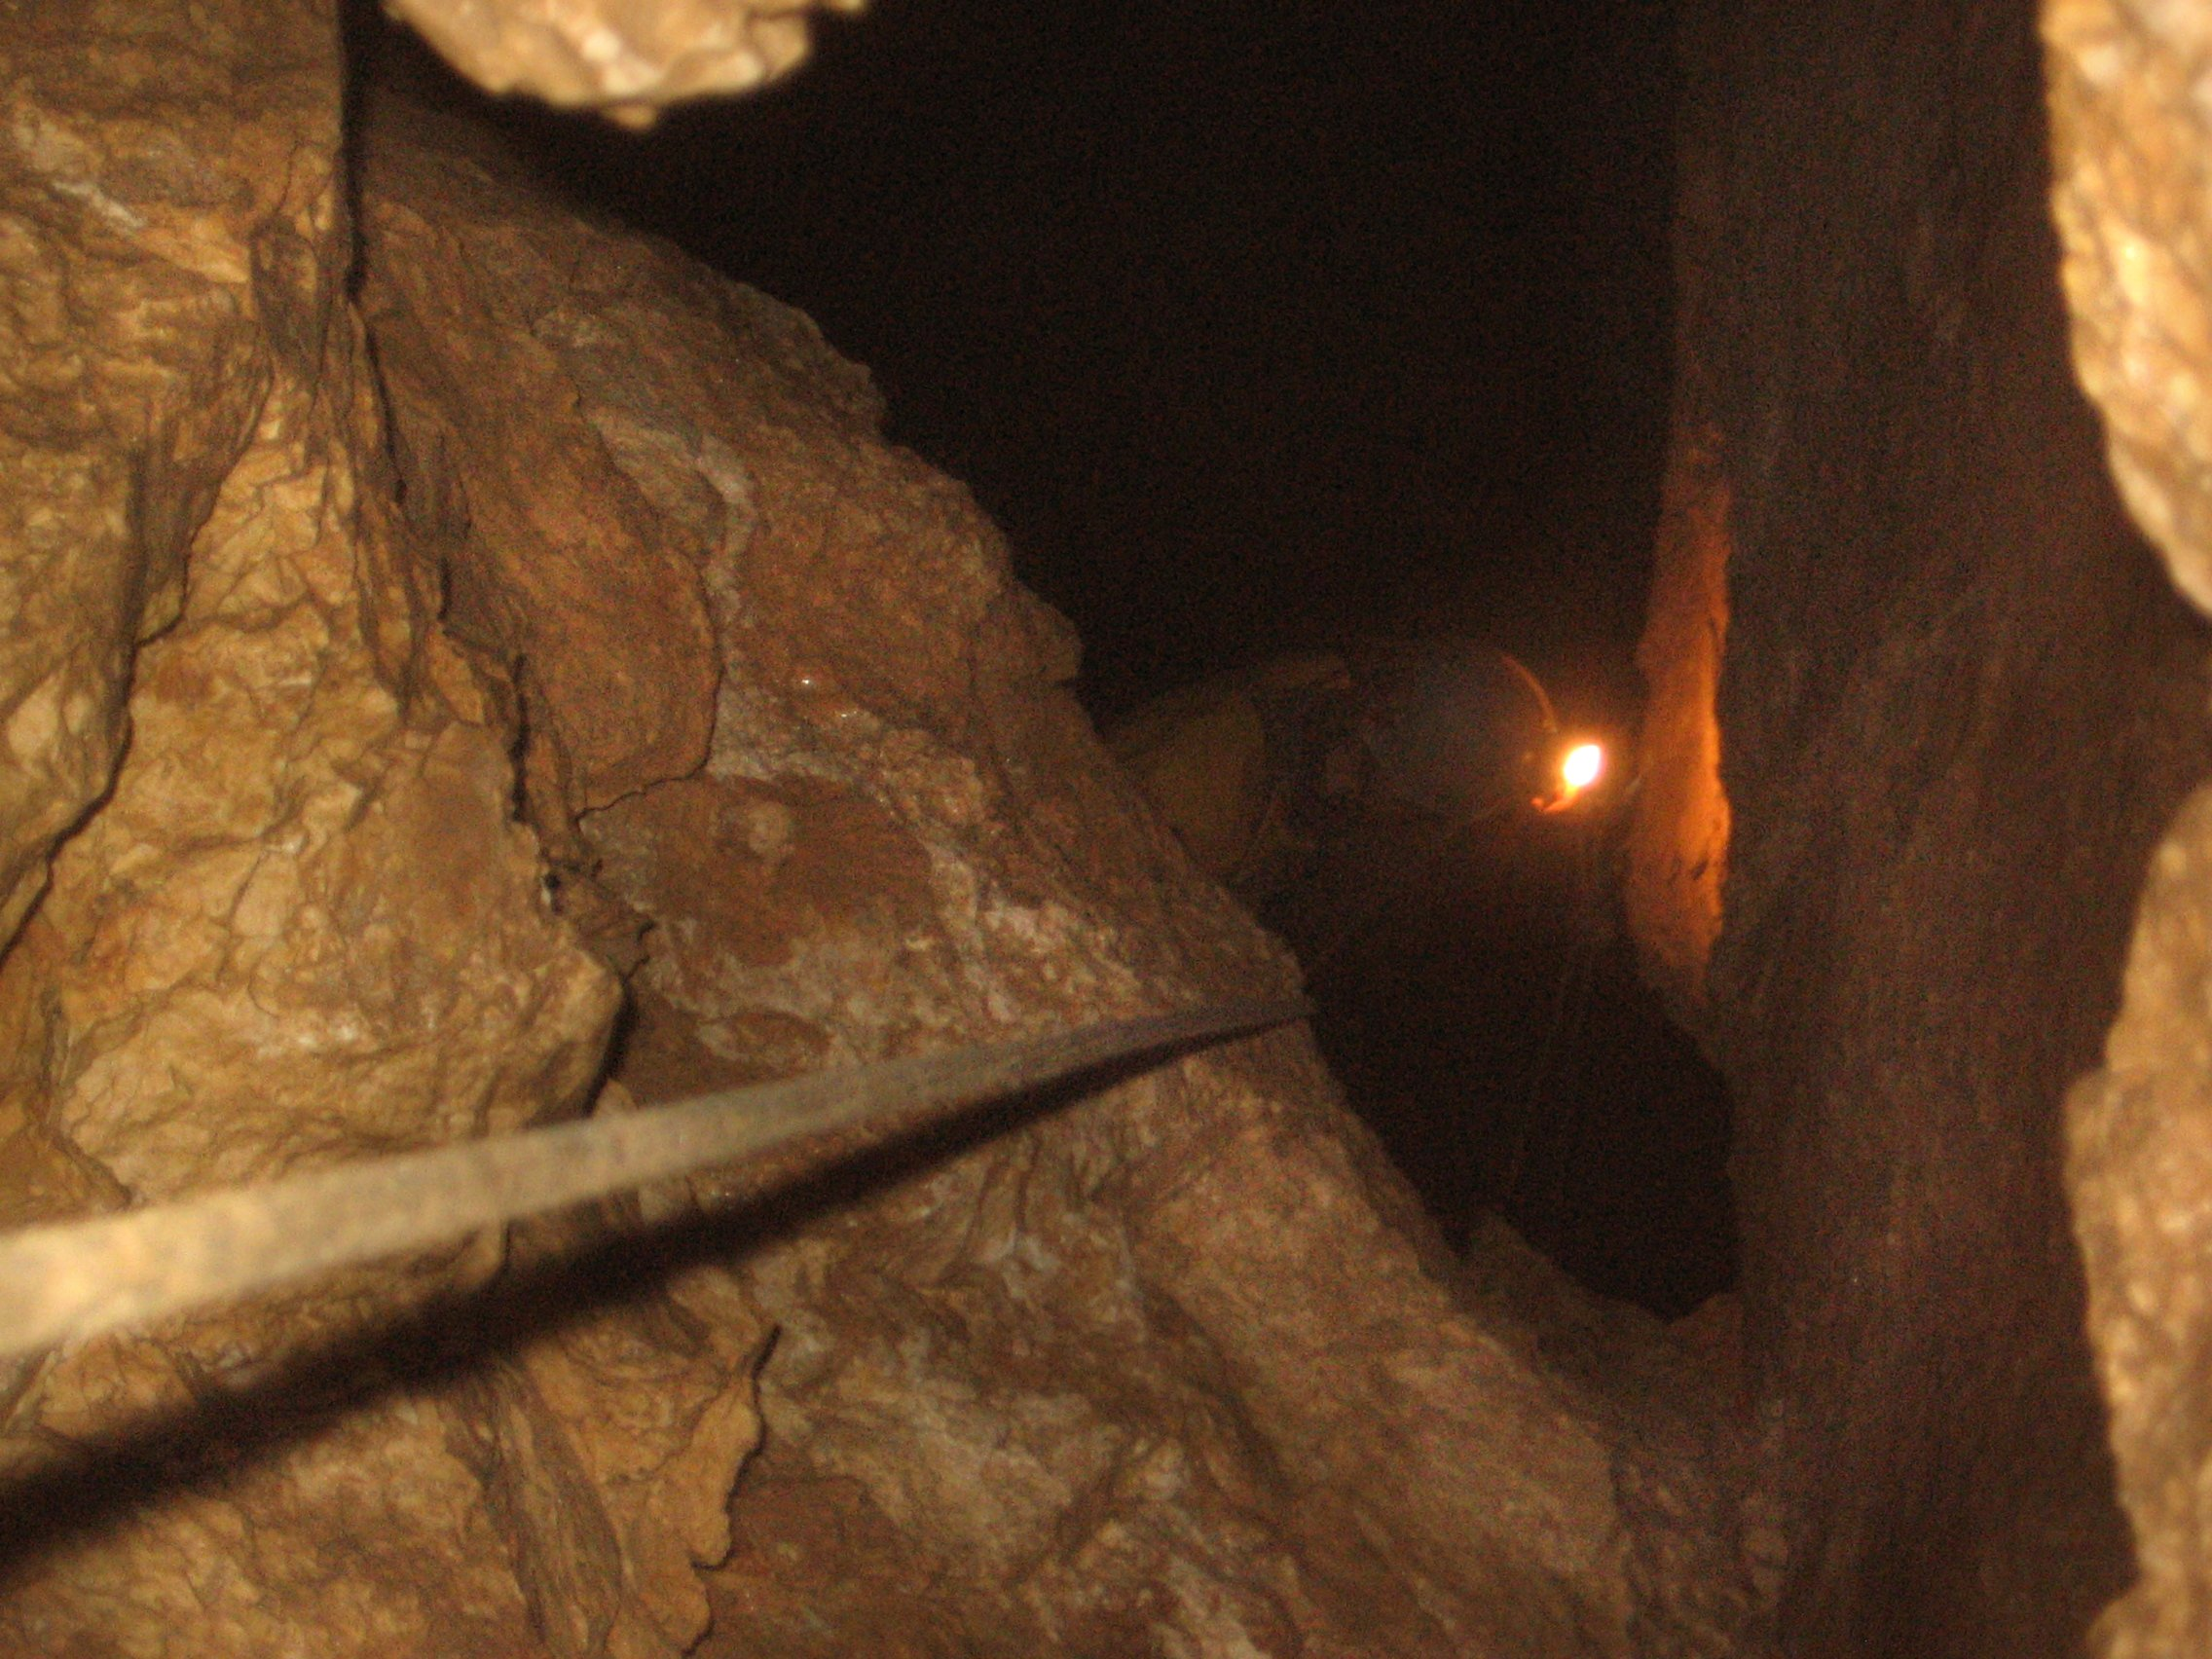
\includegraphics[width=\linewidth]{appendices/Slovenian/Jarvist Frost - canon a520 - sysmig - JC AJ trip - Andy coming up Brezno Strahov--orig.jpg}} 
 \caption{Andy Jurd coming up \protect\passage{Brezno Strahov} (Ghost pitch) in \protect\passage{M16}. \pic{Jana Čarga}}
 \label{brezno}
\end{marginfigure}

Cave –- jama\\
Entrance -– vhod\\
Pitch –- brezno\\
Chamber -– dvorana\\
Water -– voda\\
Waterfall -- slap\\
Rock, Cliff –- skala\\
Stone -- kamen\\
Rope free -- “Fraj štrik”\\
Descender –- desonder\\
Jammer –- žimar\\
Chest –- prsni\\
Foot –- nožni\\
Cowtail -- popkovina\\
Karabine –- karabin/vponka\\
Helmet -– čelada\\
Rope -– vrv/štrik\\


\subsection{Mountain dictionary}


\begin{marginfigure}
\checkoddpage \ifoddpage \forcerectofloat \else \forceversofloat \fi
\centering
 \frame{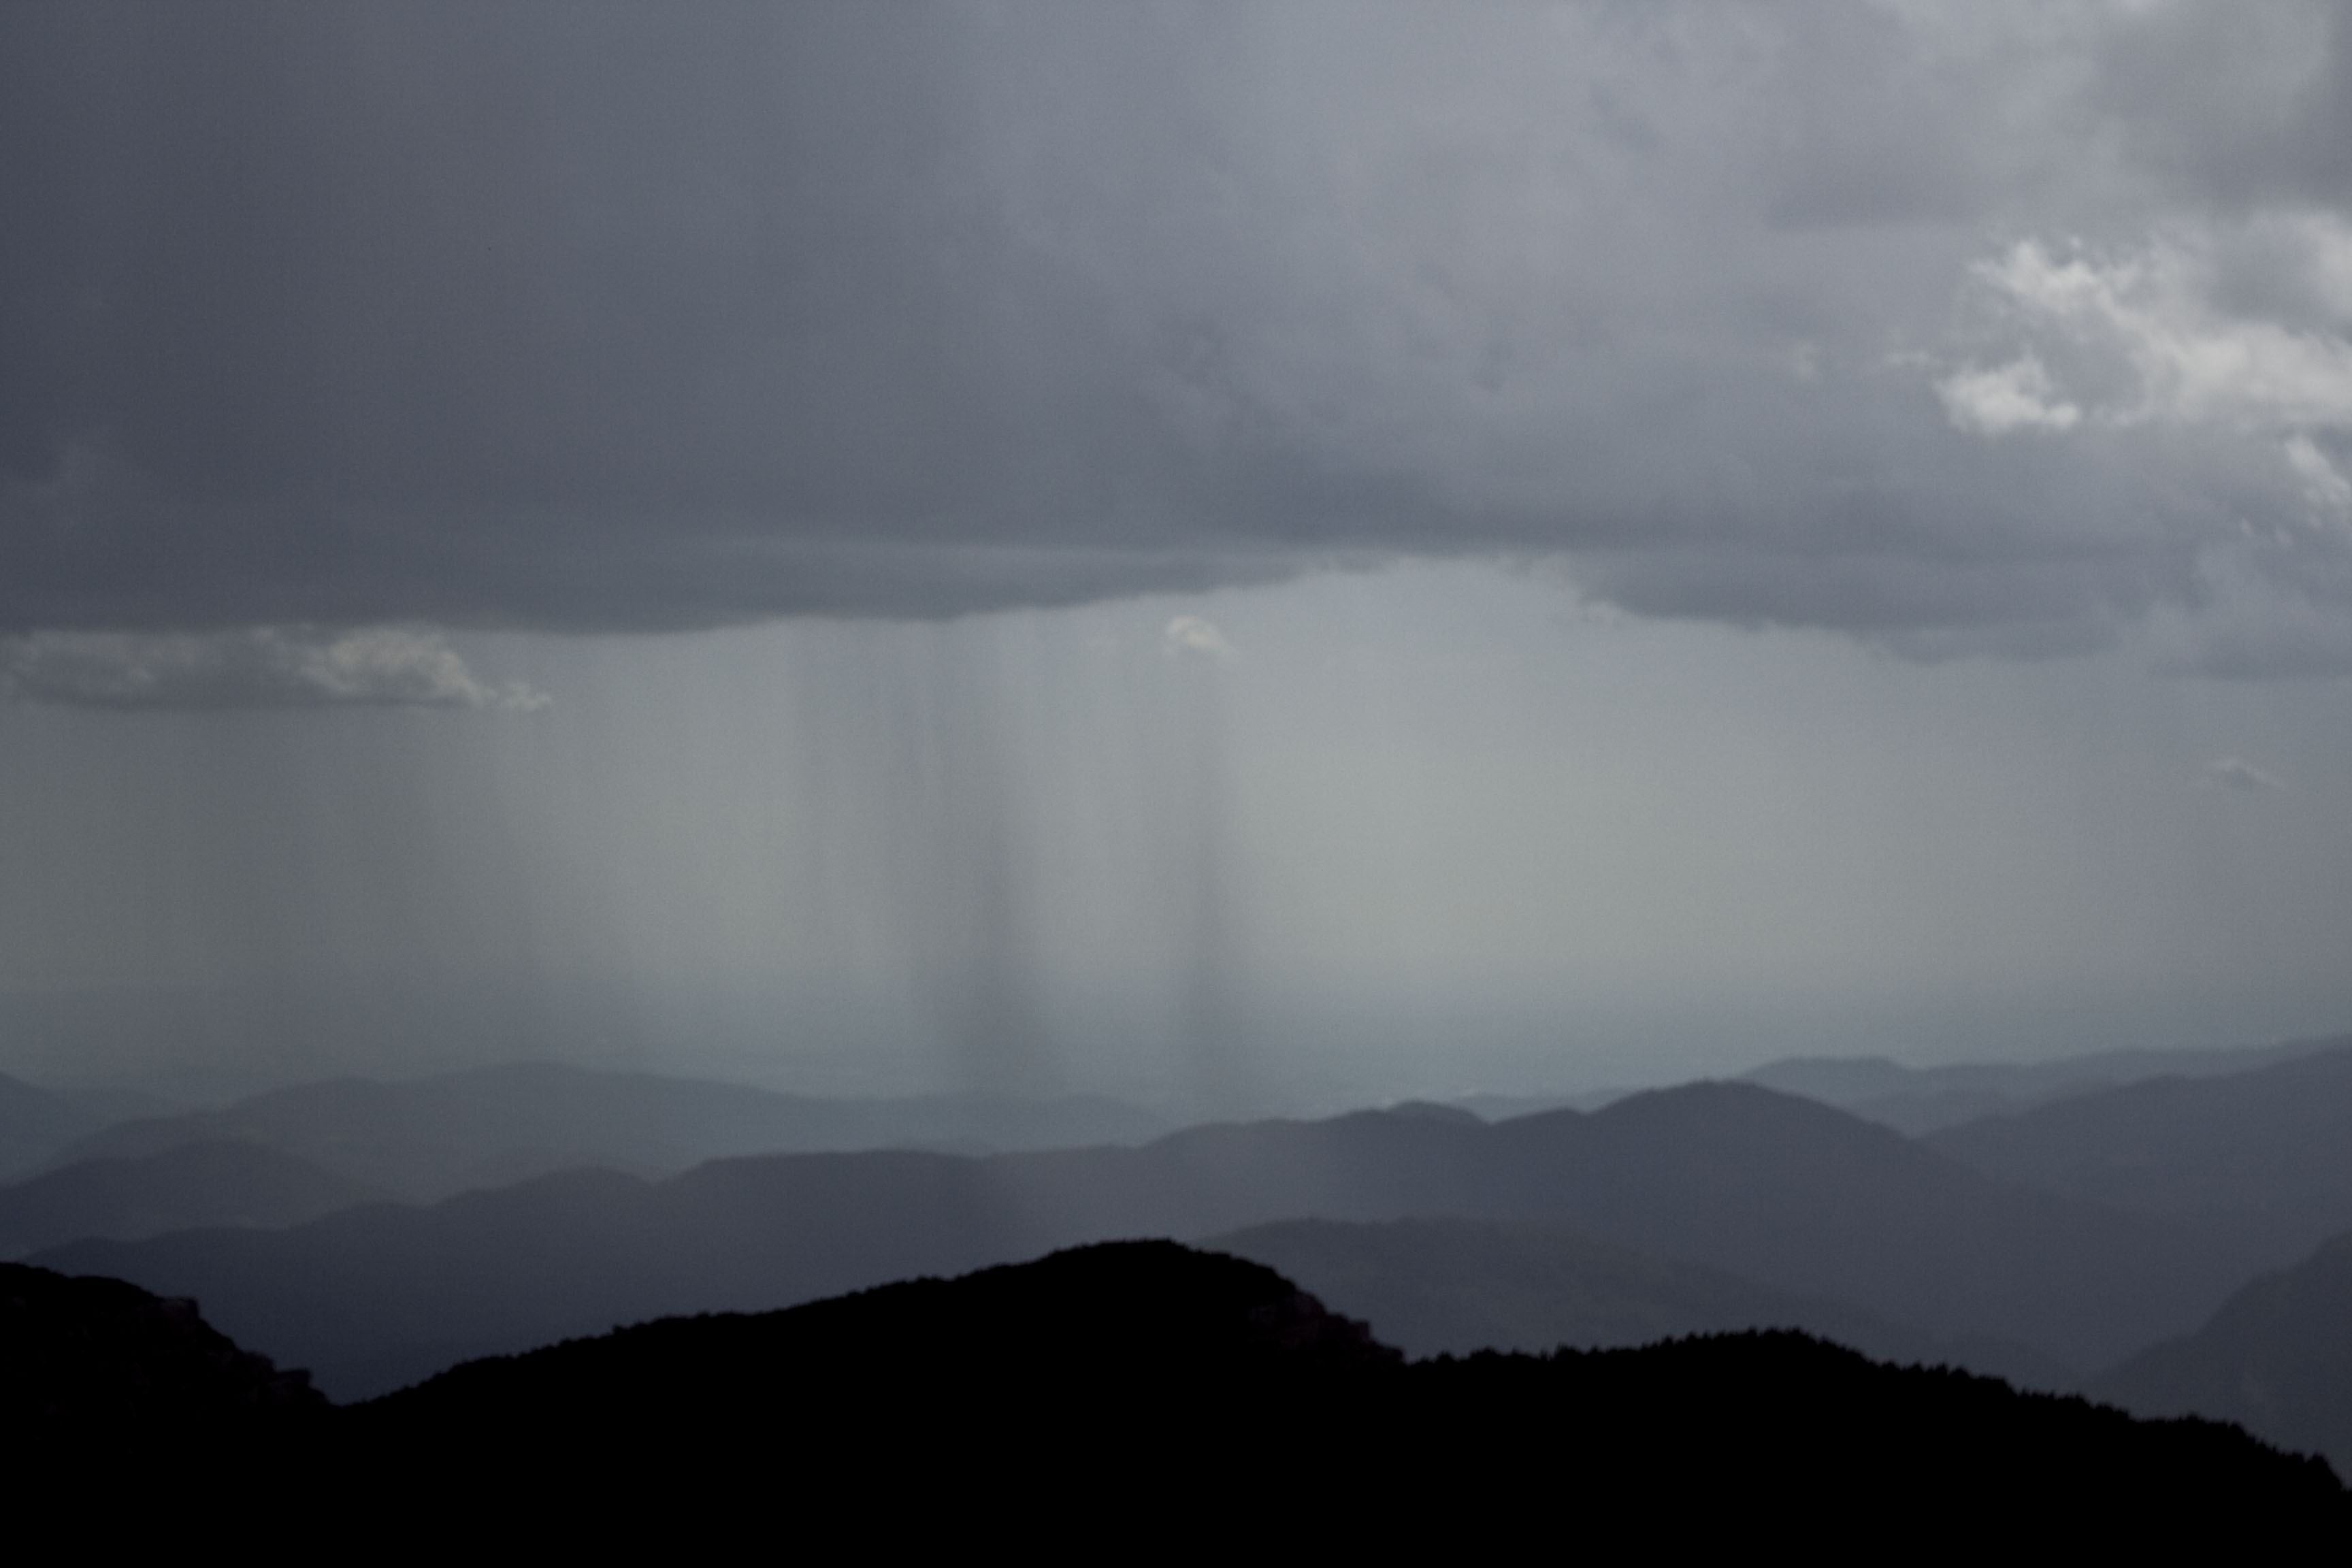
\includegraphics[width=\linewidth]{appendices/Slovenian/2009-Jana Carga - Canon 350d - 219_1--orig.jpg}} 
 \caption{Rain (dež) in the mountains. \pic{Jana Čarga}}
 \label{dež}
\end{marginfigure}

Mountain -– gora\\
Hill –- hrib\\
Valley -– dolina\\
River -– reka\\
Stream -- potok\\
Goat –- koza\\
Cow –- krava\\
Tent -- šotor\\
Sleeping bag -– spalna vreča\\
Wind –- veter\\
Rain -- dež\\
Help –- na pomoč\\

\subsection{Basic phrases}

\begin{marginfigure}
\checkoddpage \ifoddpage \forcerectofloat \else \forceversofloat \fi
\centering
 \frame{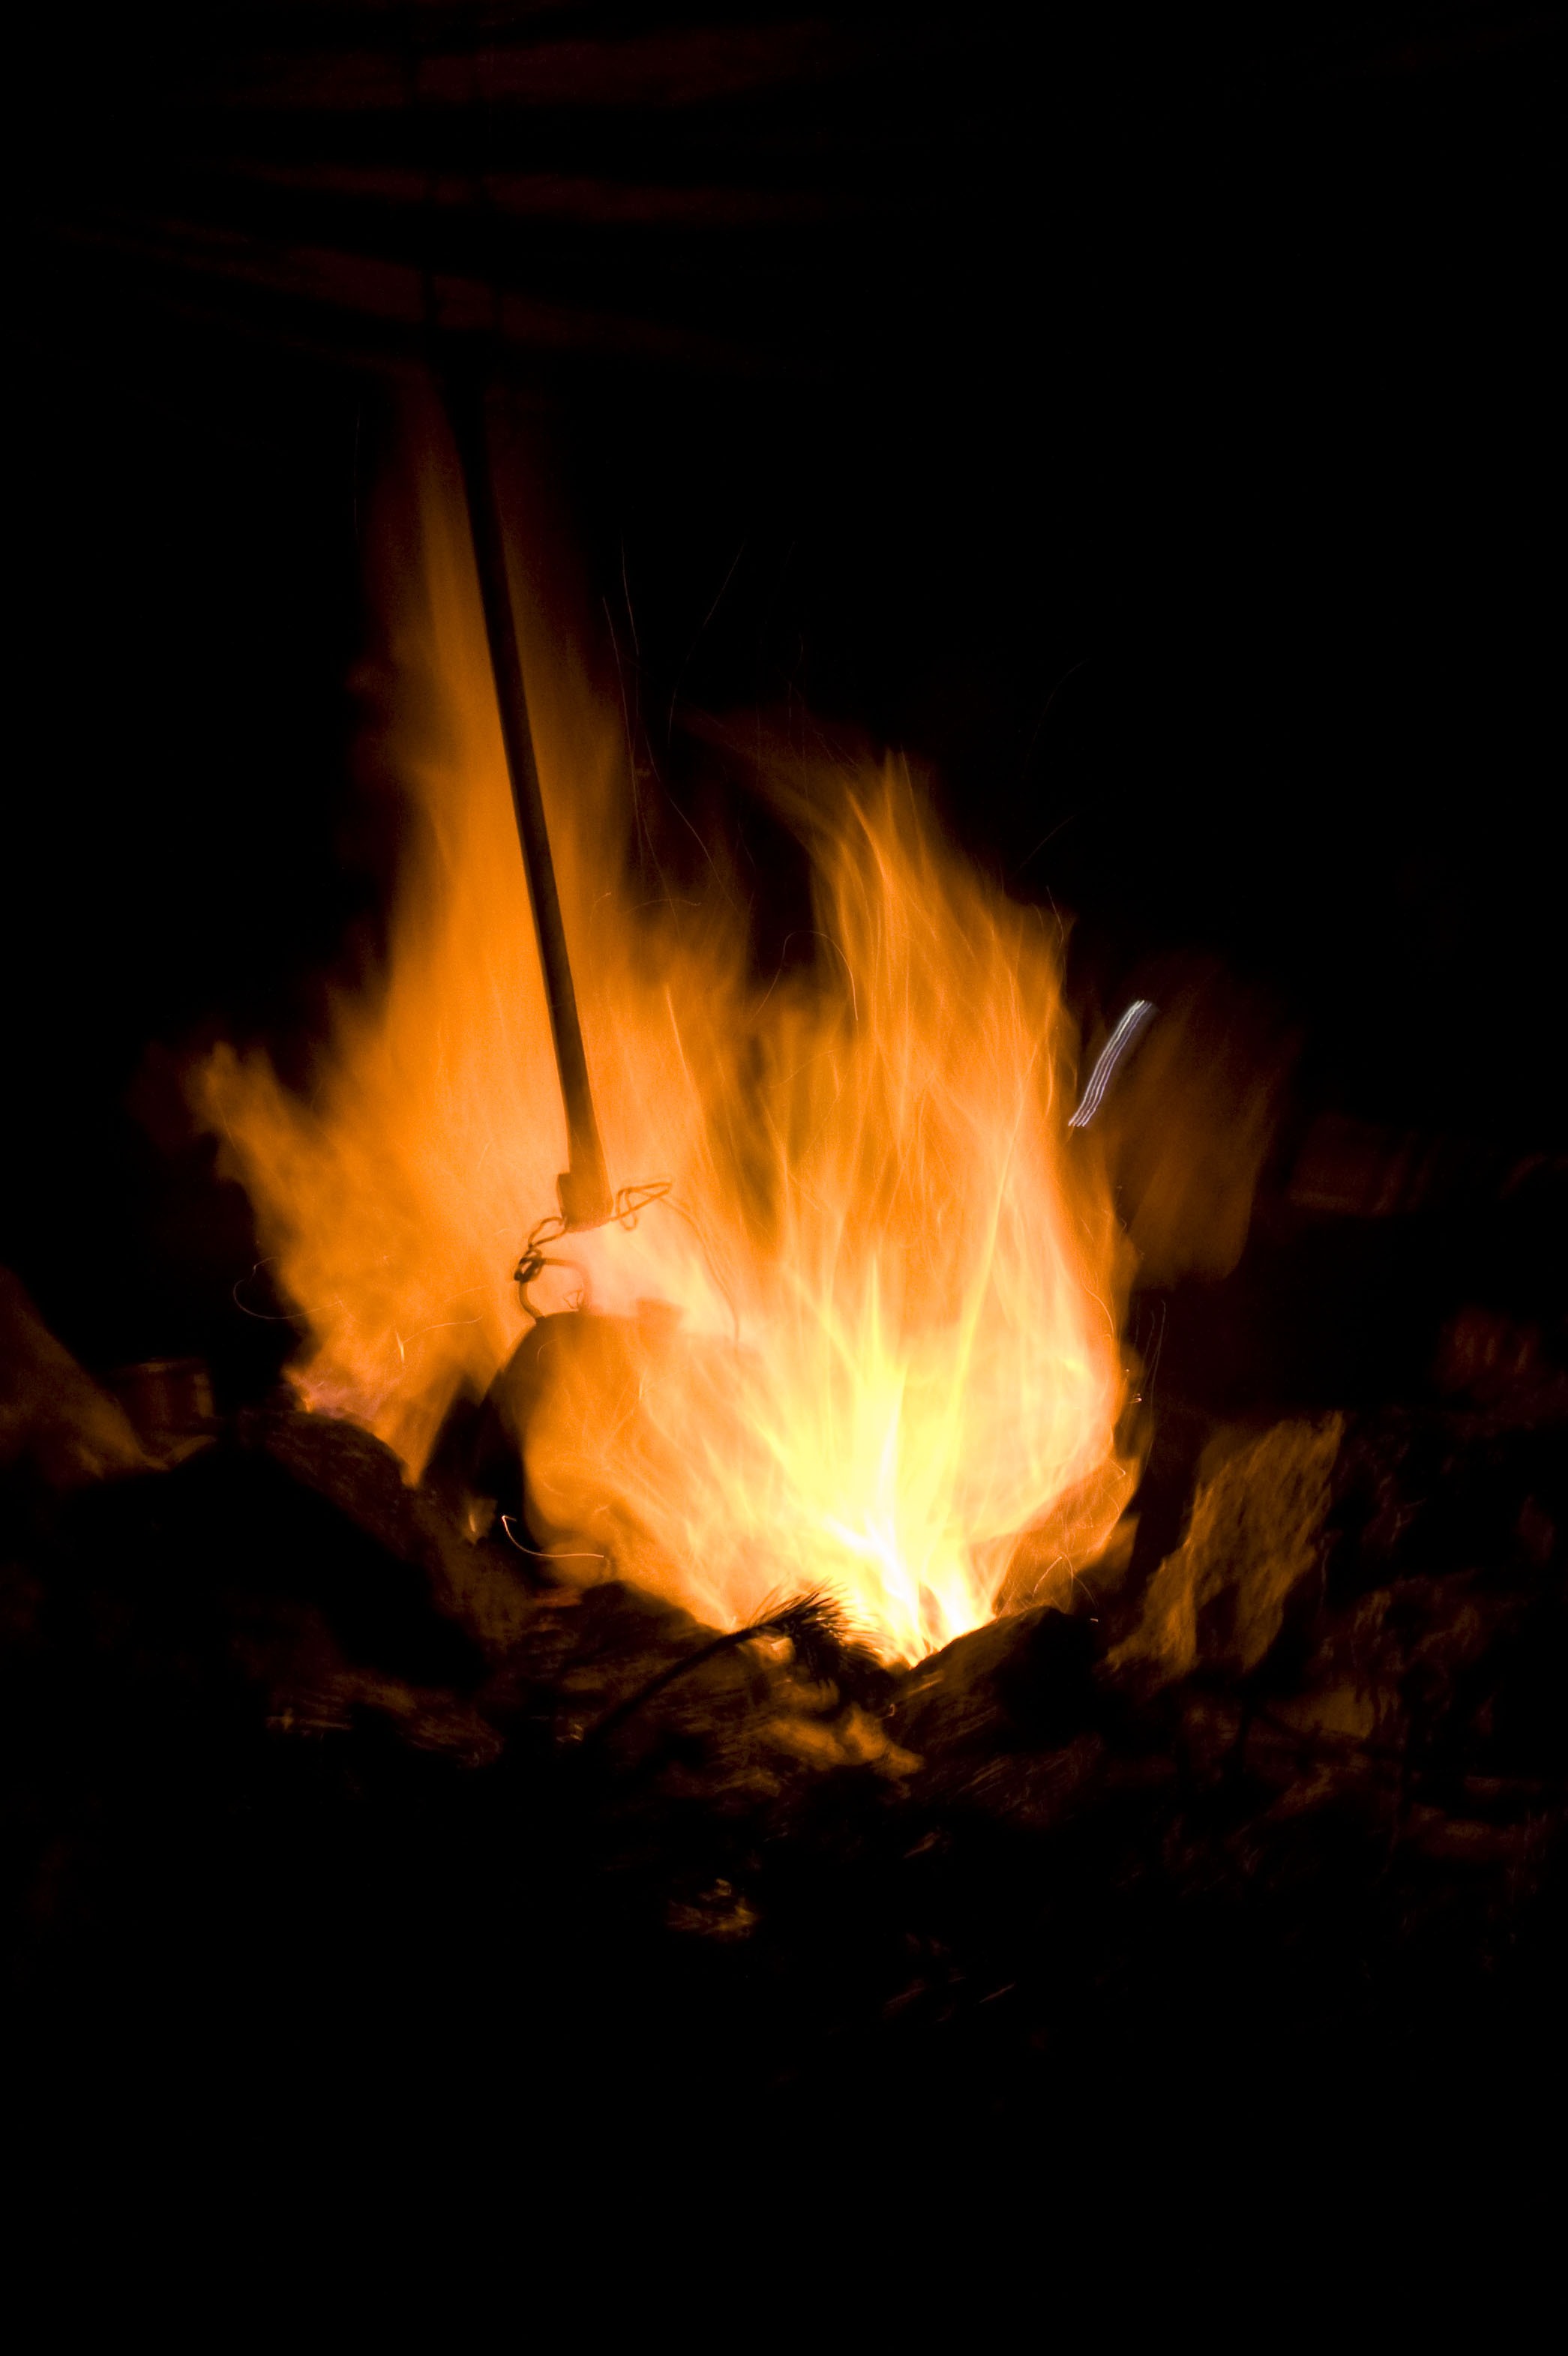
\includegraphics[width=\linewidth]{appendices/Slovenian/2009-Jana Carga - Canon 350d - 143_1--orig.jpg}} 
 \caption{Once sunset is finished the night will typically feature a round of hot drinks in the bivi. Afterwards people will head to bed. They'll all say lahko noč (good night) on their way out - though the pronunciation of 'lahko' will vary considerably. \pic{Jana Čarga}}
 \label{nighttime tea}
\end{marginfigure}

Hello. -- Živijo.\\
How are you? -- Kako si?\\
Fine, thank you. -- Hvala, dobro.\\
What is your name? -- Kako ti je ime? (inf) / Kako vam je ime? (pol)\\
My name is\ldots{} -- Ime mi je \ldots{}\\
Nice to meet you. -- Lepo, da sva se spoznala\\
Please. -- Prosim.\\
Thank you. -- Hvala.\\
You're welcome. -- Dobrodošli.\\
Yes. -- Da. / Ja.\\
No. -- Ne.\\
Excuse me.  -- Oprostite.\\
I'm sorry. -- Oprostite.\\
have trouble speaking Slovenian. -- Slabo govorim slovensko.\\
Do you speak English? -- Govorite angleško?\\
Is there someone here who speaks English?  -- Je tukaj kdo, ki govori angleško?\\
Help! -- Na pomoč!\\
Look out! -- Pazi!\\
Good day. -- Dober dan.\\
Good morning. -- Dobro jutro.\\
Good evening. -- Dober večer.\\
Good night. -- Lahko noč.\\
I don't understand.  -- Ne razumem.\\
Where is the toilet? -- Kje je stranišče?\\
I need your help. -- Potrebujem vašo pomoč.\\
I'm lost. -- Izgubil sem se.\\
I'm sick. -- Bolan sem./Slabo mi je.\\
I've been injured.  -- Poškodoval sem se.\\
I need a doctor. -- Potrebujem zdravnika.\\
Can I use your phone? -- Lahko uporabim vaš telefon?\\


\subsection{Numbers}


\begin{marginfigure}
\checkoddpage \ifoddpage \forcerectofloat \else \forceversofloat \fi
\centering
 \frame{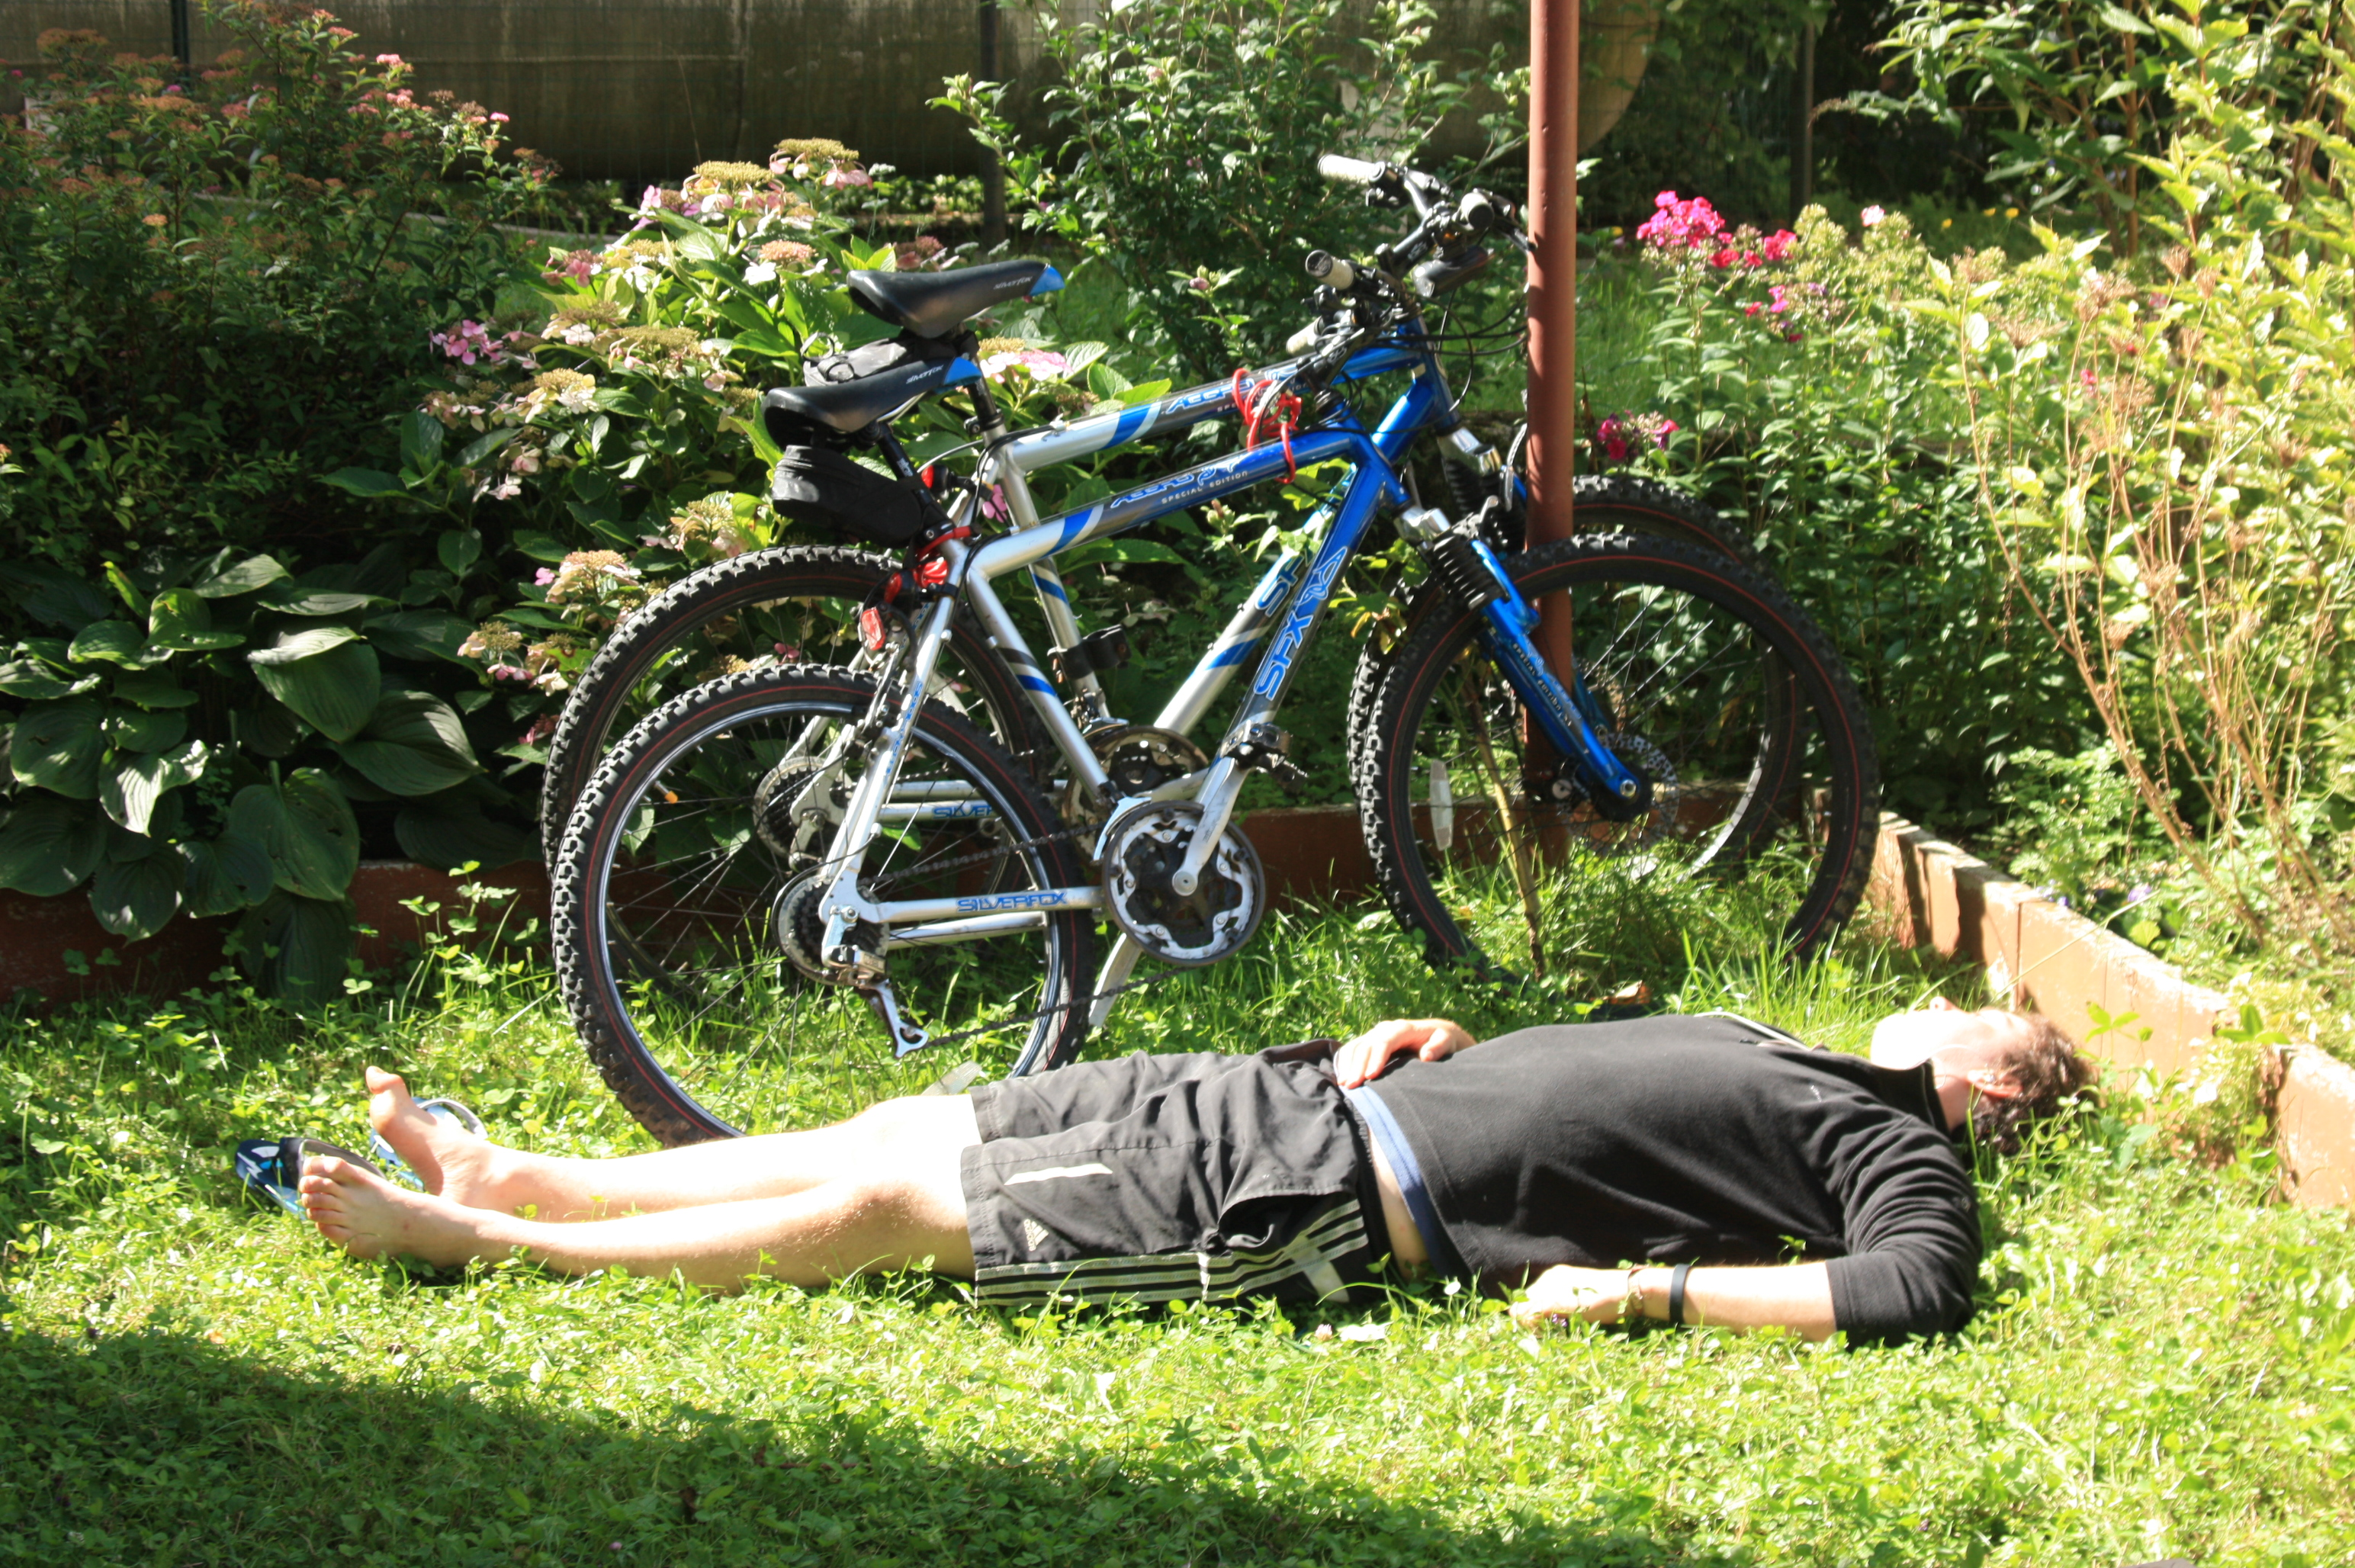
\includegraphics[width=\linewidth]{appendices/Slovenian/2011-08-12-09.59.58-Gergely Ambrus-Canon450D-IMG_1399-Mountain Derig--orig.jpg}} 
 \caption{Two bicycles (dve kolesi) that were used to cycle from Ravne to Tolmin. \pic{Gergely Ambrus}}
 \label{kolo}
\end{marginfigure}

Number -- številka\\
Half --  pol\\
Less -- manj\\
More -- več\\
1 ena\\
2 dva\\
3 tri\\
4 štiri\\
5 pet\\
6 šest\\
7 sedem\\
8 osem\\
9 devet\\
10 deset\\
20 dvajset\\
30 trideset\\
40 štirideset\\
50 petdeset\\
60 šestdeset\\
70 sedemdeset\\
80 osemdeset\\
90 devetdeset\\
100 sto\\
1000 tisoč\\
1,000,000 milijon\\

\subsection{Time}


\begin{marginfigure}
\checkoddpage \ifoddpage \forcerectofloat \else \forceversofloat \fi
\centering
 \frame{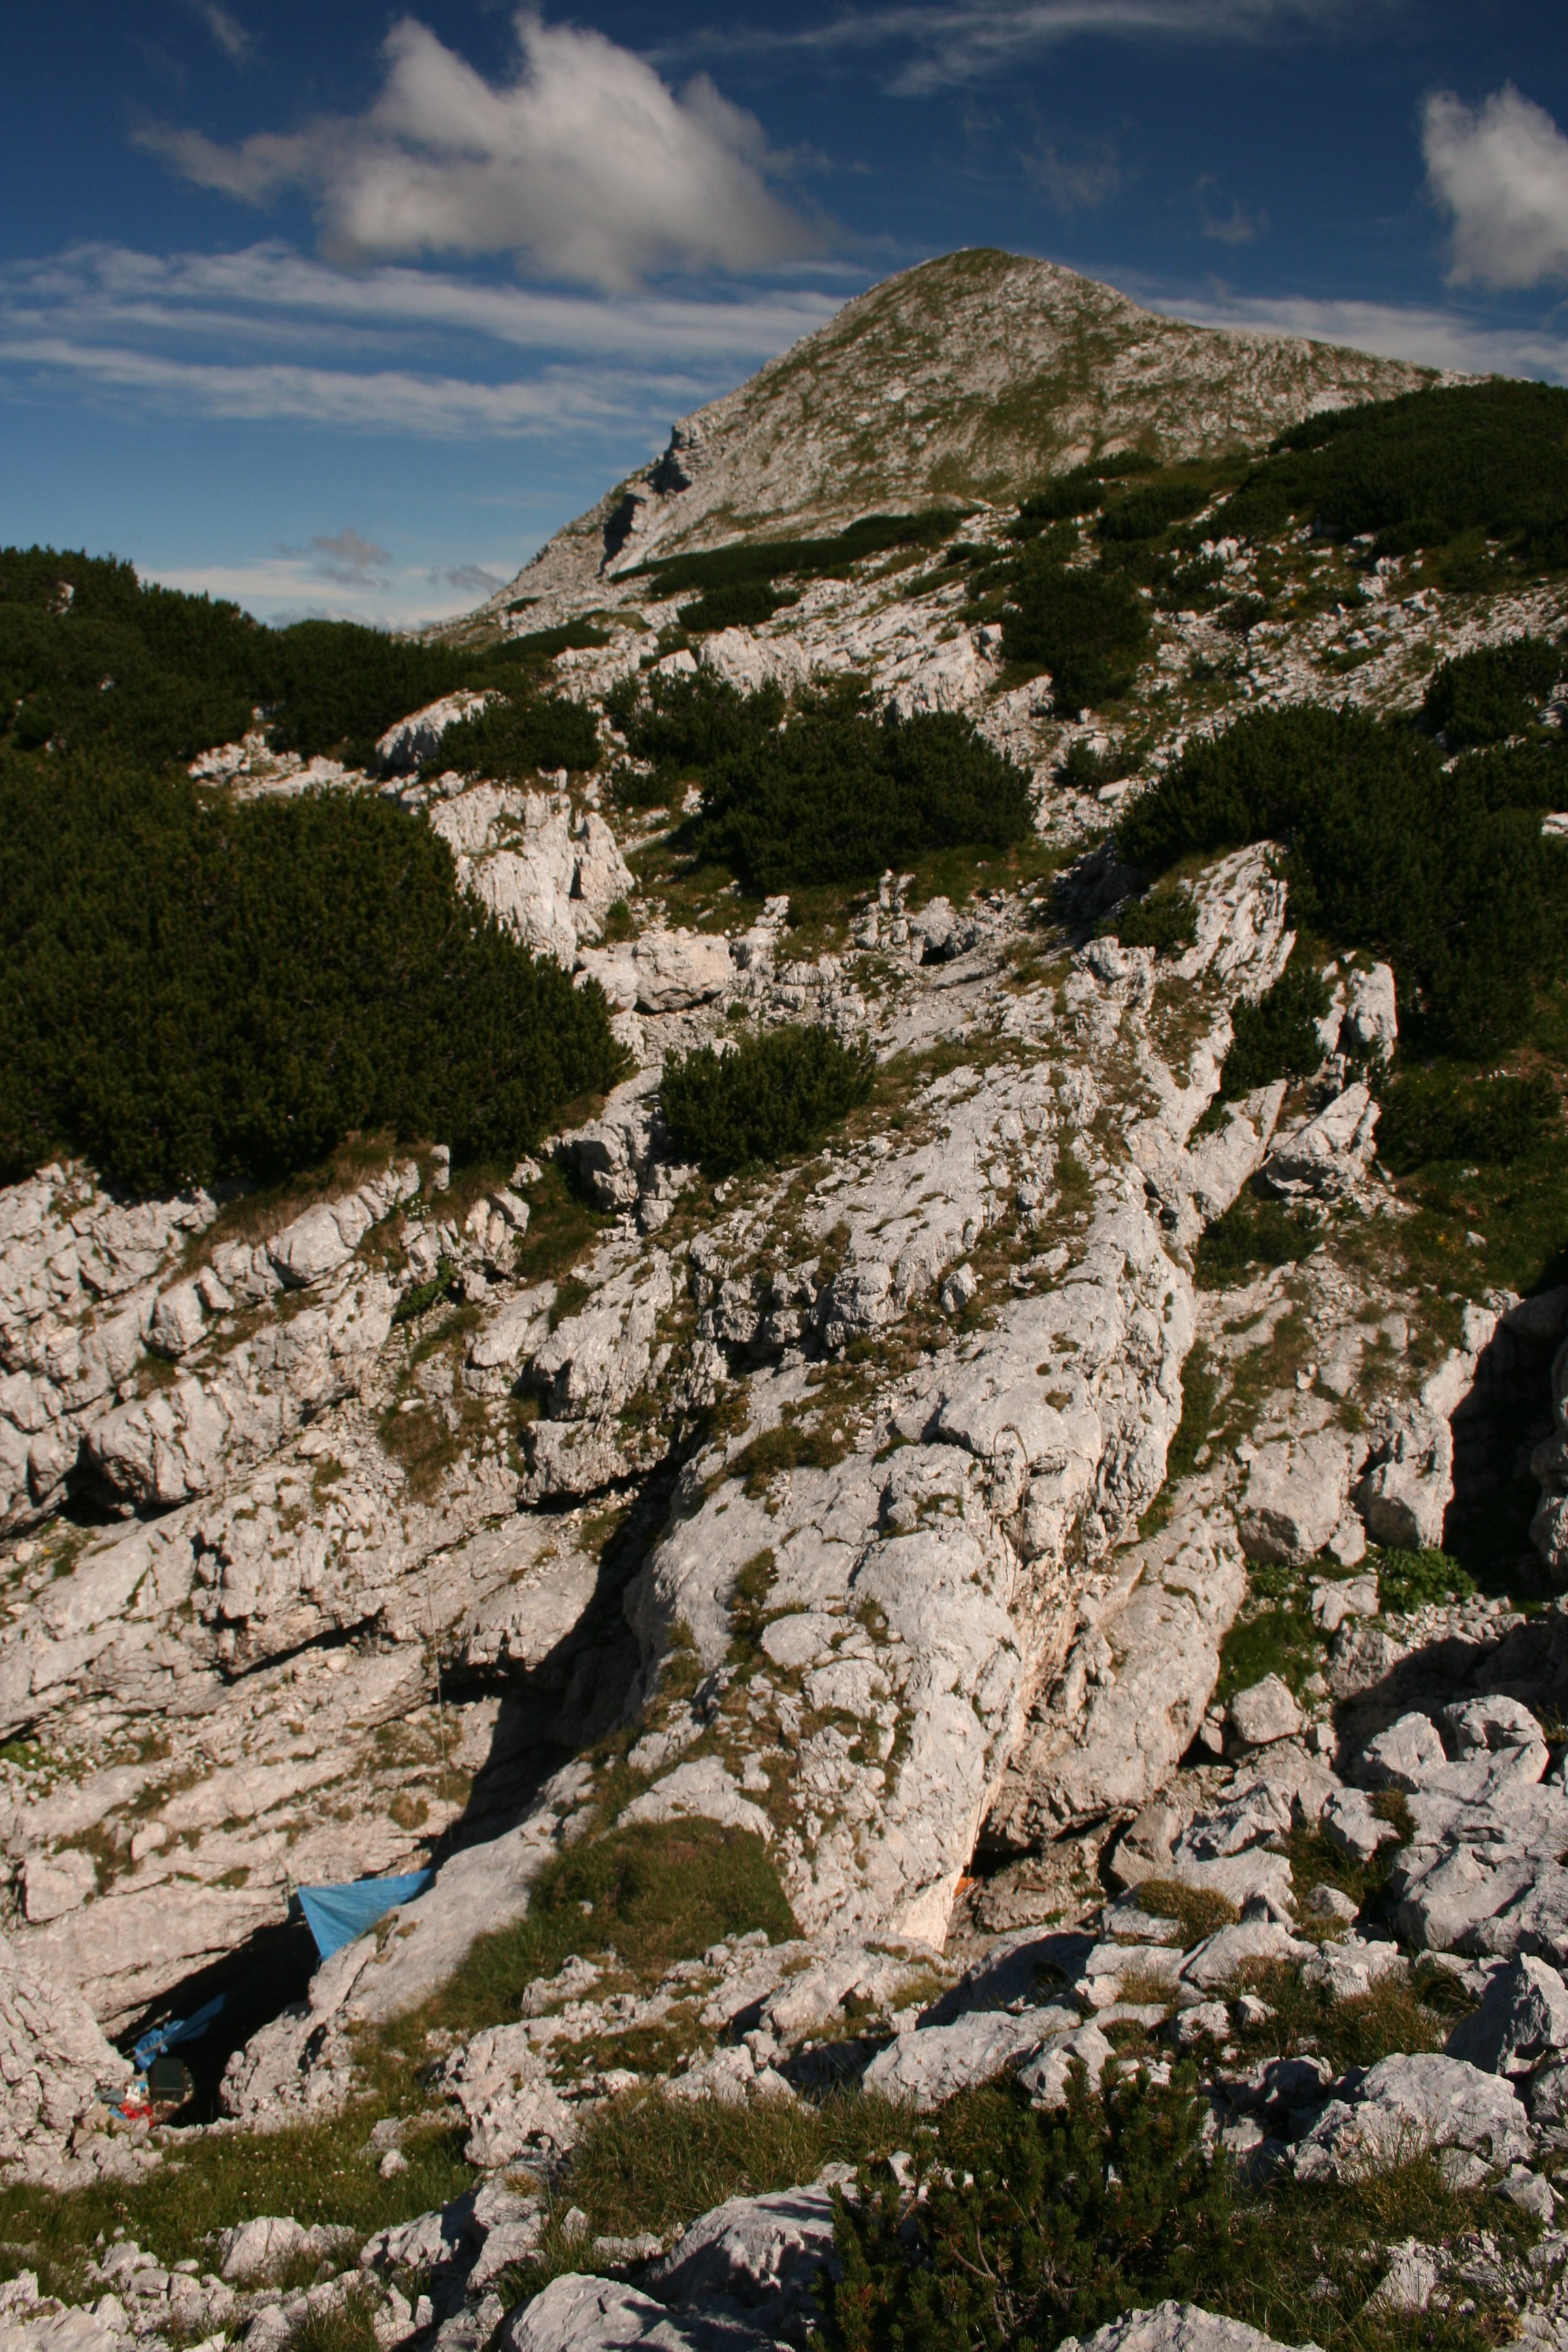
\includegraphics[width=\linewidth]{appendices/Slovenian/Jana Carga - Canon 350D - img_2999 bivi on a sunny late morning--orig.jpg}} 
 \caption{The rock bridge over the bivi, late in the morning (jutro). \pic{Jana Čarga}}
 \label{jutro}
\end{marginfigure}


\begin{marginfigure}
\checkoddpage \ifoddpage \forcerectofloat \else \forceversofloat \fi
\centering
 \frame{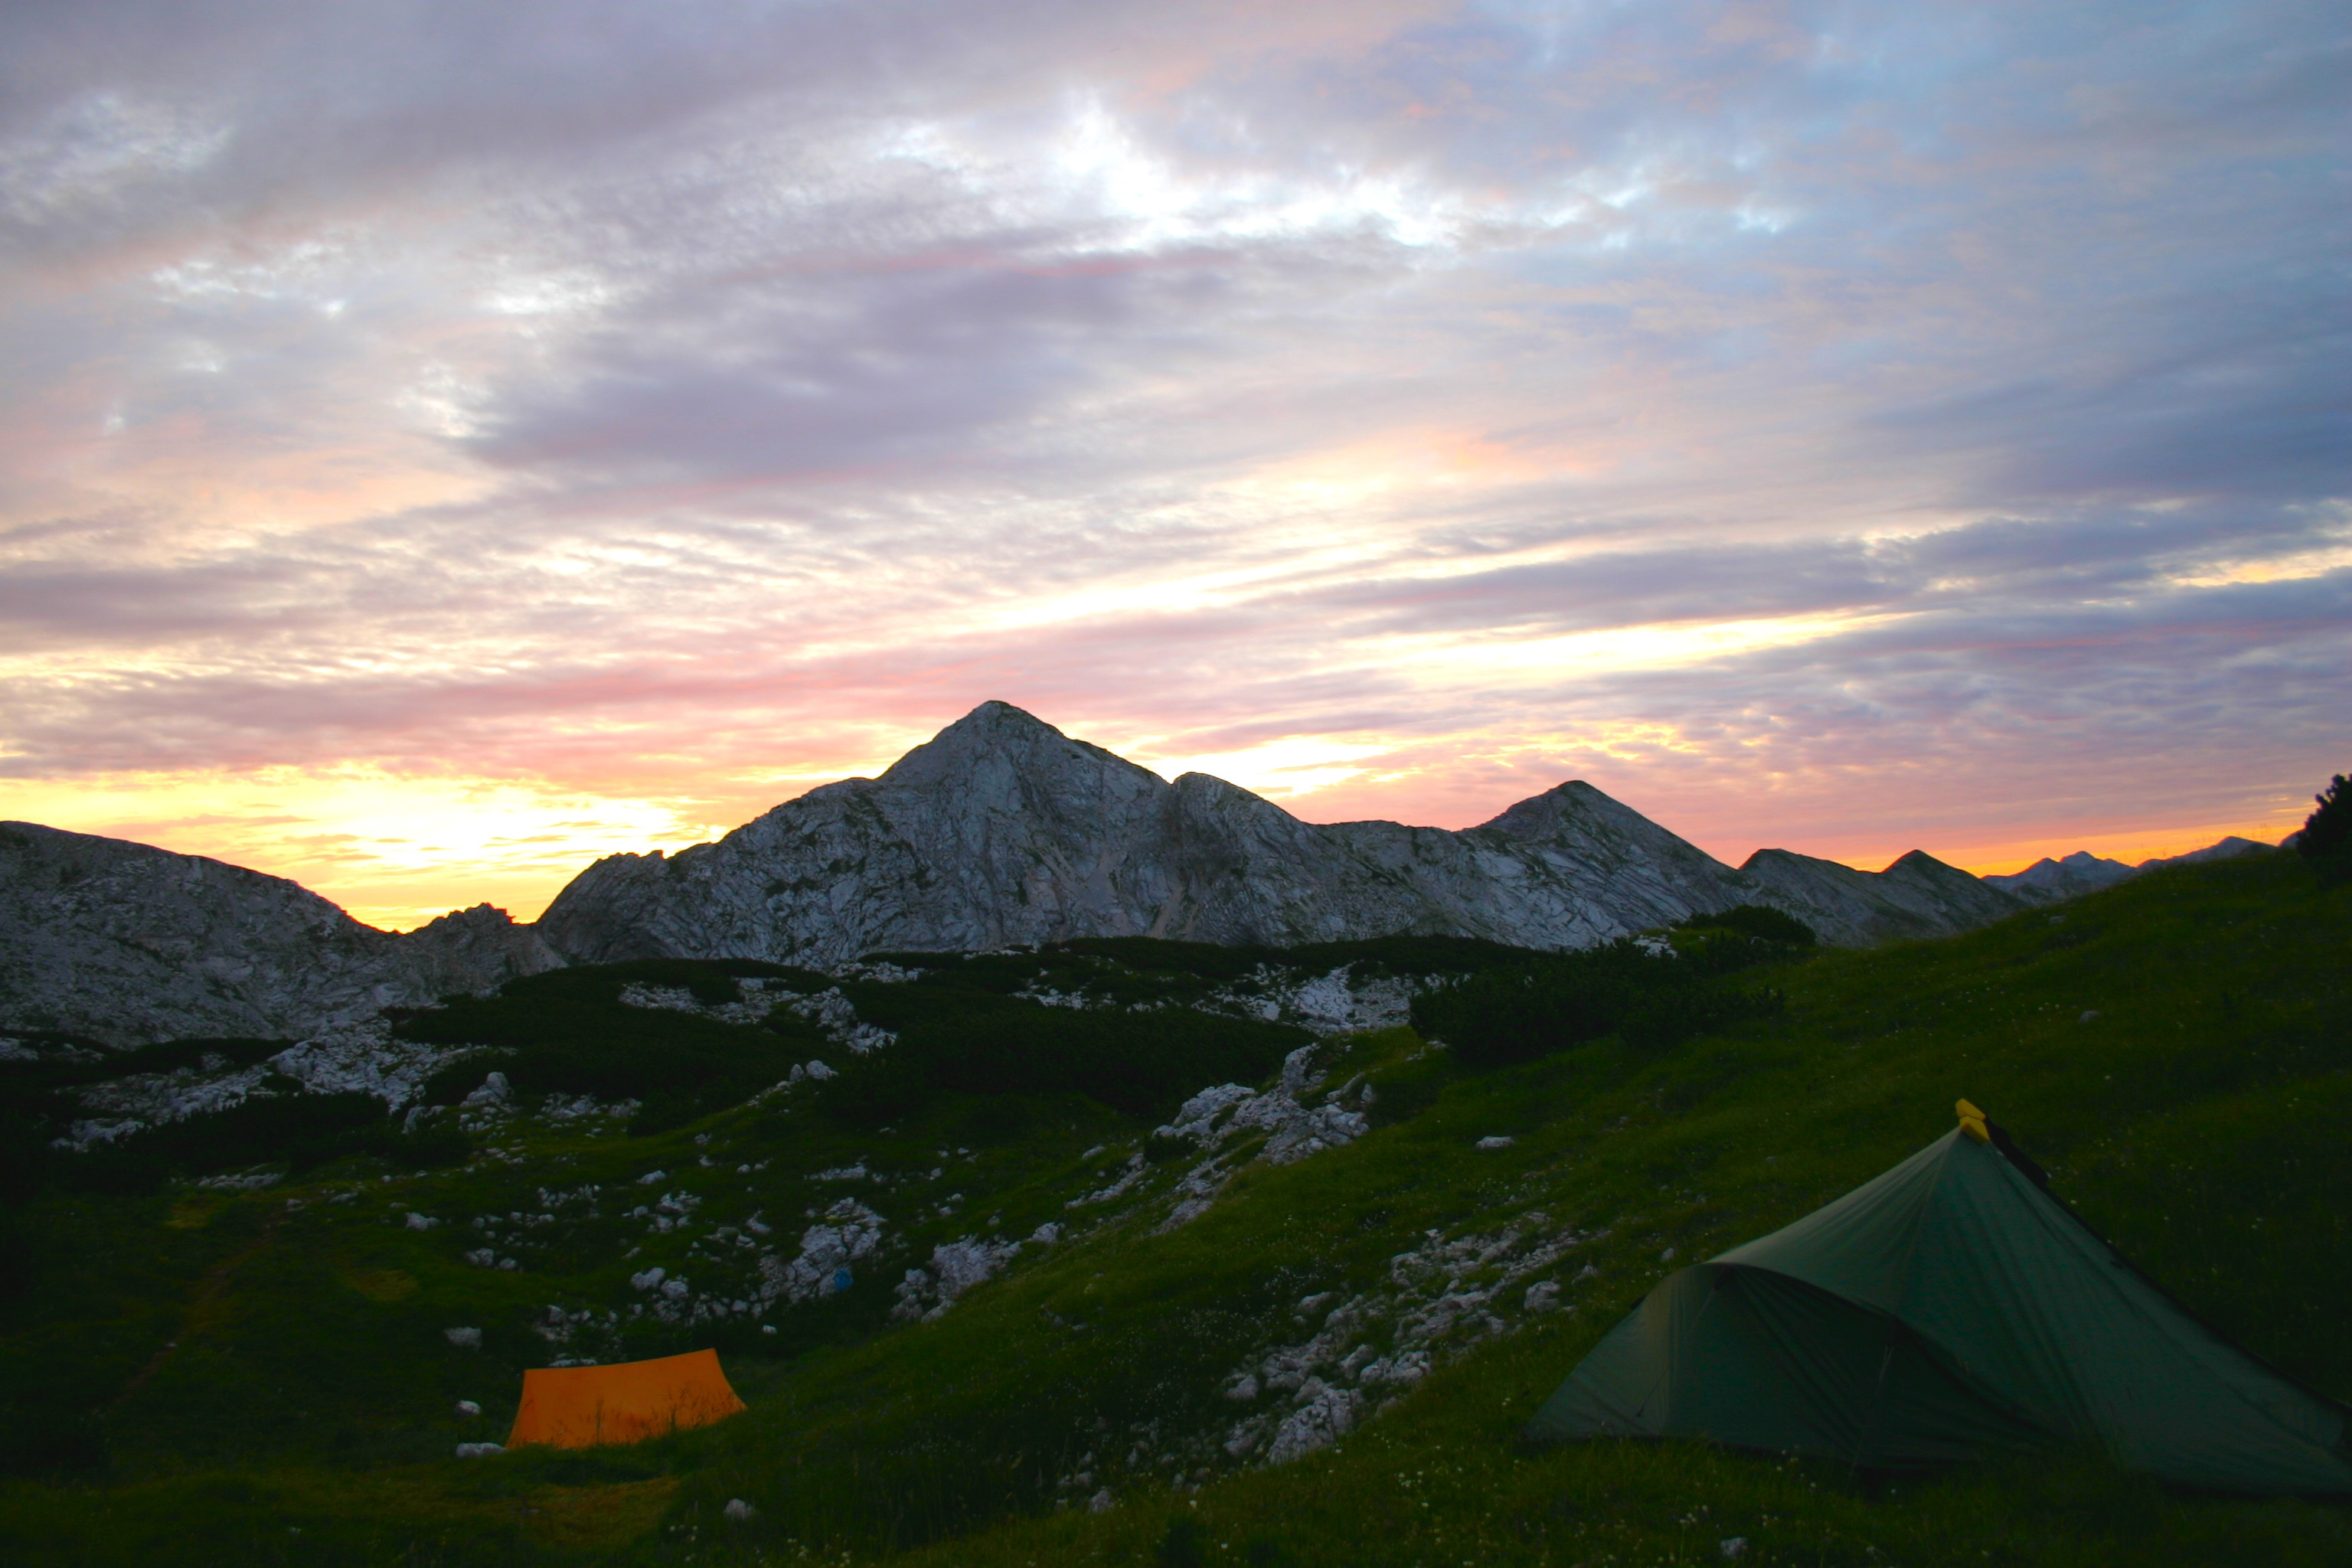
\includegraphics[width=\linewidth]{appendices/Slovenian/2009-08-17-11.13.23 - Tharatorn Supasiti - Plateau at dawn 1 - IMG_5386-1--orig.jpg}} 
 \caption{The plateau at dawn. \pic{Tharatorn Supasiti}}
 \label{rain}
\end{marginfigure}

now -- sedaj\\
later -- kasneje\\
before -- pred\\
morning -- jutro\\
noon -- poldan\\
afternoon -- popoldne\\
evening -- večer\\
night -- noč\\
Today -- danes\\
Yesterday -- včeraj\\
Tomorrow -- jutri\\
This week -- ta teden\\
Last week -- prejšnji teden\\
Next week -- naslednji teden\\

\subsection{Time of the day}

one o'clock AM -- ena zjutraj\\
two o'clock AM -- dve zjutraj\\
noon -- poldan\\
one o'clock PM -- ena popoldne\\
two o'clock PM -- dve popoldne\\
midnight -– polnoč\\

\subsection{Duration}

MINUTE(s)\\ 
1 minuta / 2 minuti/ 3,4 minute/ 5-100 minut\\
HOURS(s) \\
1 ura/ 2 uri/ 3,4 ure/ 5-100 ur\\
DAY(s) \\
1 dan/ 2 dneva/ 3,4 dnevi/ 5-100 dni\\
WEEK(s) \\
1 teden/ 2 tedna/ 3,4 tedni/ 5-100 tednov\\
MONTH(s) \\
1 mesec/ 2 meseca/ 3,4 meseci/ 5-100 mesecev\\
YEAR(s) \\
1 leto/ 2 leti/ 3,4 leta/ 5-100 let\\

\subsection{Days}

Monday -- ponedeljek\\
Tuesday -- torek\\
Wednesday -- sreda\\
Thursday -- četrtek\\
Friday -- petek\\
Saturday -- sobota\\
Sunday -- nedelja\\

\subsection{Months}


\begin{marginfigure}
\checkoddpage \ifoddpage \forcerectofloat \else \forceversofloat \fi
\centering
 \frame{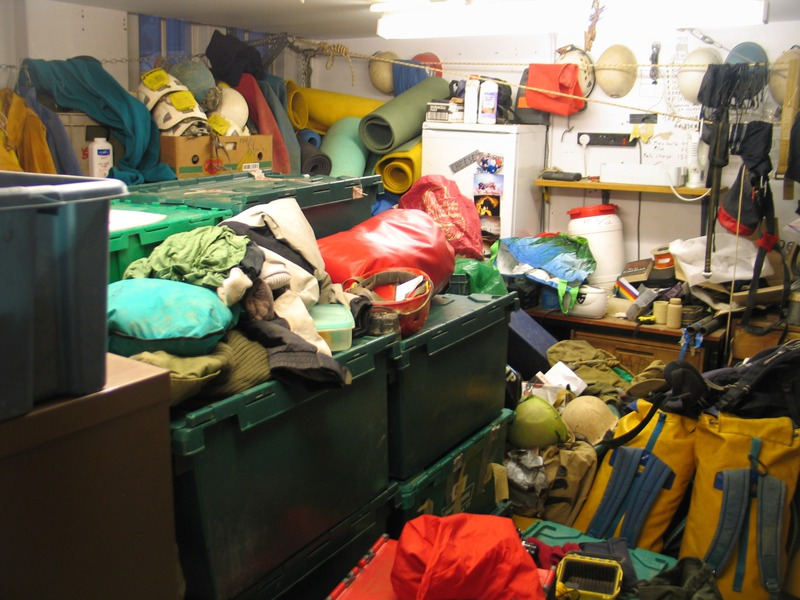
\includegraphics[width=\linewidth]{appendices/Slovenian/2011-08-14-19.10.45-Jarvist Frost-CanonG5-IMG_0203 - many crates safely back in stores--orig.jpg}} 
 \caption{Caving gear comes in almost every colour. \pic{Jarvist Frost}}
 \label{colourful gear}
\end{marginfigure}

January -- januar / prosinec\\
February -- februar / svečan\\
March -- marec / sušec\\
April -- april / mali traven\\
May -- maj / veliki traven\\
June -- junij / rožnik\\
July -- julij / mali srpan\\
August -- avgust / veliki srpan\\
September -- september / kimavec\\
October -- oktober / vinotok\\
November -- november / listopad\\
December -- december / gruden\\

\subsection{Colours}

black -- črna\\
white -- bela\\
gray -- siva\\
red -- rdeča\\
blue -- modra\\
cyan -- sinja\\
yellow -- rumena\\
green -- zelena\\
orange -- oranžna\\
purple -- vijolična, škrlatna\\
brown -- rjava\\
pink -- roza\\

\subsection{Transportation}

How much is a ticket? -- Kakšna je cena vozovnice?\\
One ticket, please. -- Eno vozovnico, prosim.\\
Where does this train/bus go? -- Kam gre ta vlak/avtobus?\\
Does this train/bus stop in\ldots{} -- Ali ta vlak/avtobus ustavi v\ldots{}\\
When does the train/bus leave? -- Kdaj odide vlak/avtobus?\\
When will this train/bus arrive? -- Kdaj pride vlak/avtobus?\\
Bus -- avtobus\\ 
Train -- vlak\\
bus station -- avtobusna postaja\\
train station -- železniška postaja\\
waiting room -- čakalnica\\
ticket sale -- prodaja vozovnic\\
Binary -- peron\\
Ticket -- karta/vozovnica\\
Seat -- sedež\\
Coach -- vagon\\
Conductor -- sprevodnik\\
express train -- ekspres vlak\\
intercity train -- IC vlak\\
Slovenian Railways -- Slovenske železnice (SŽ)\\

\begin{marginfigure}
\checkoddpage \ifoddpage \forcerectofloat \else \forceversofloat \fi
\centering
 \frame{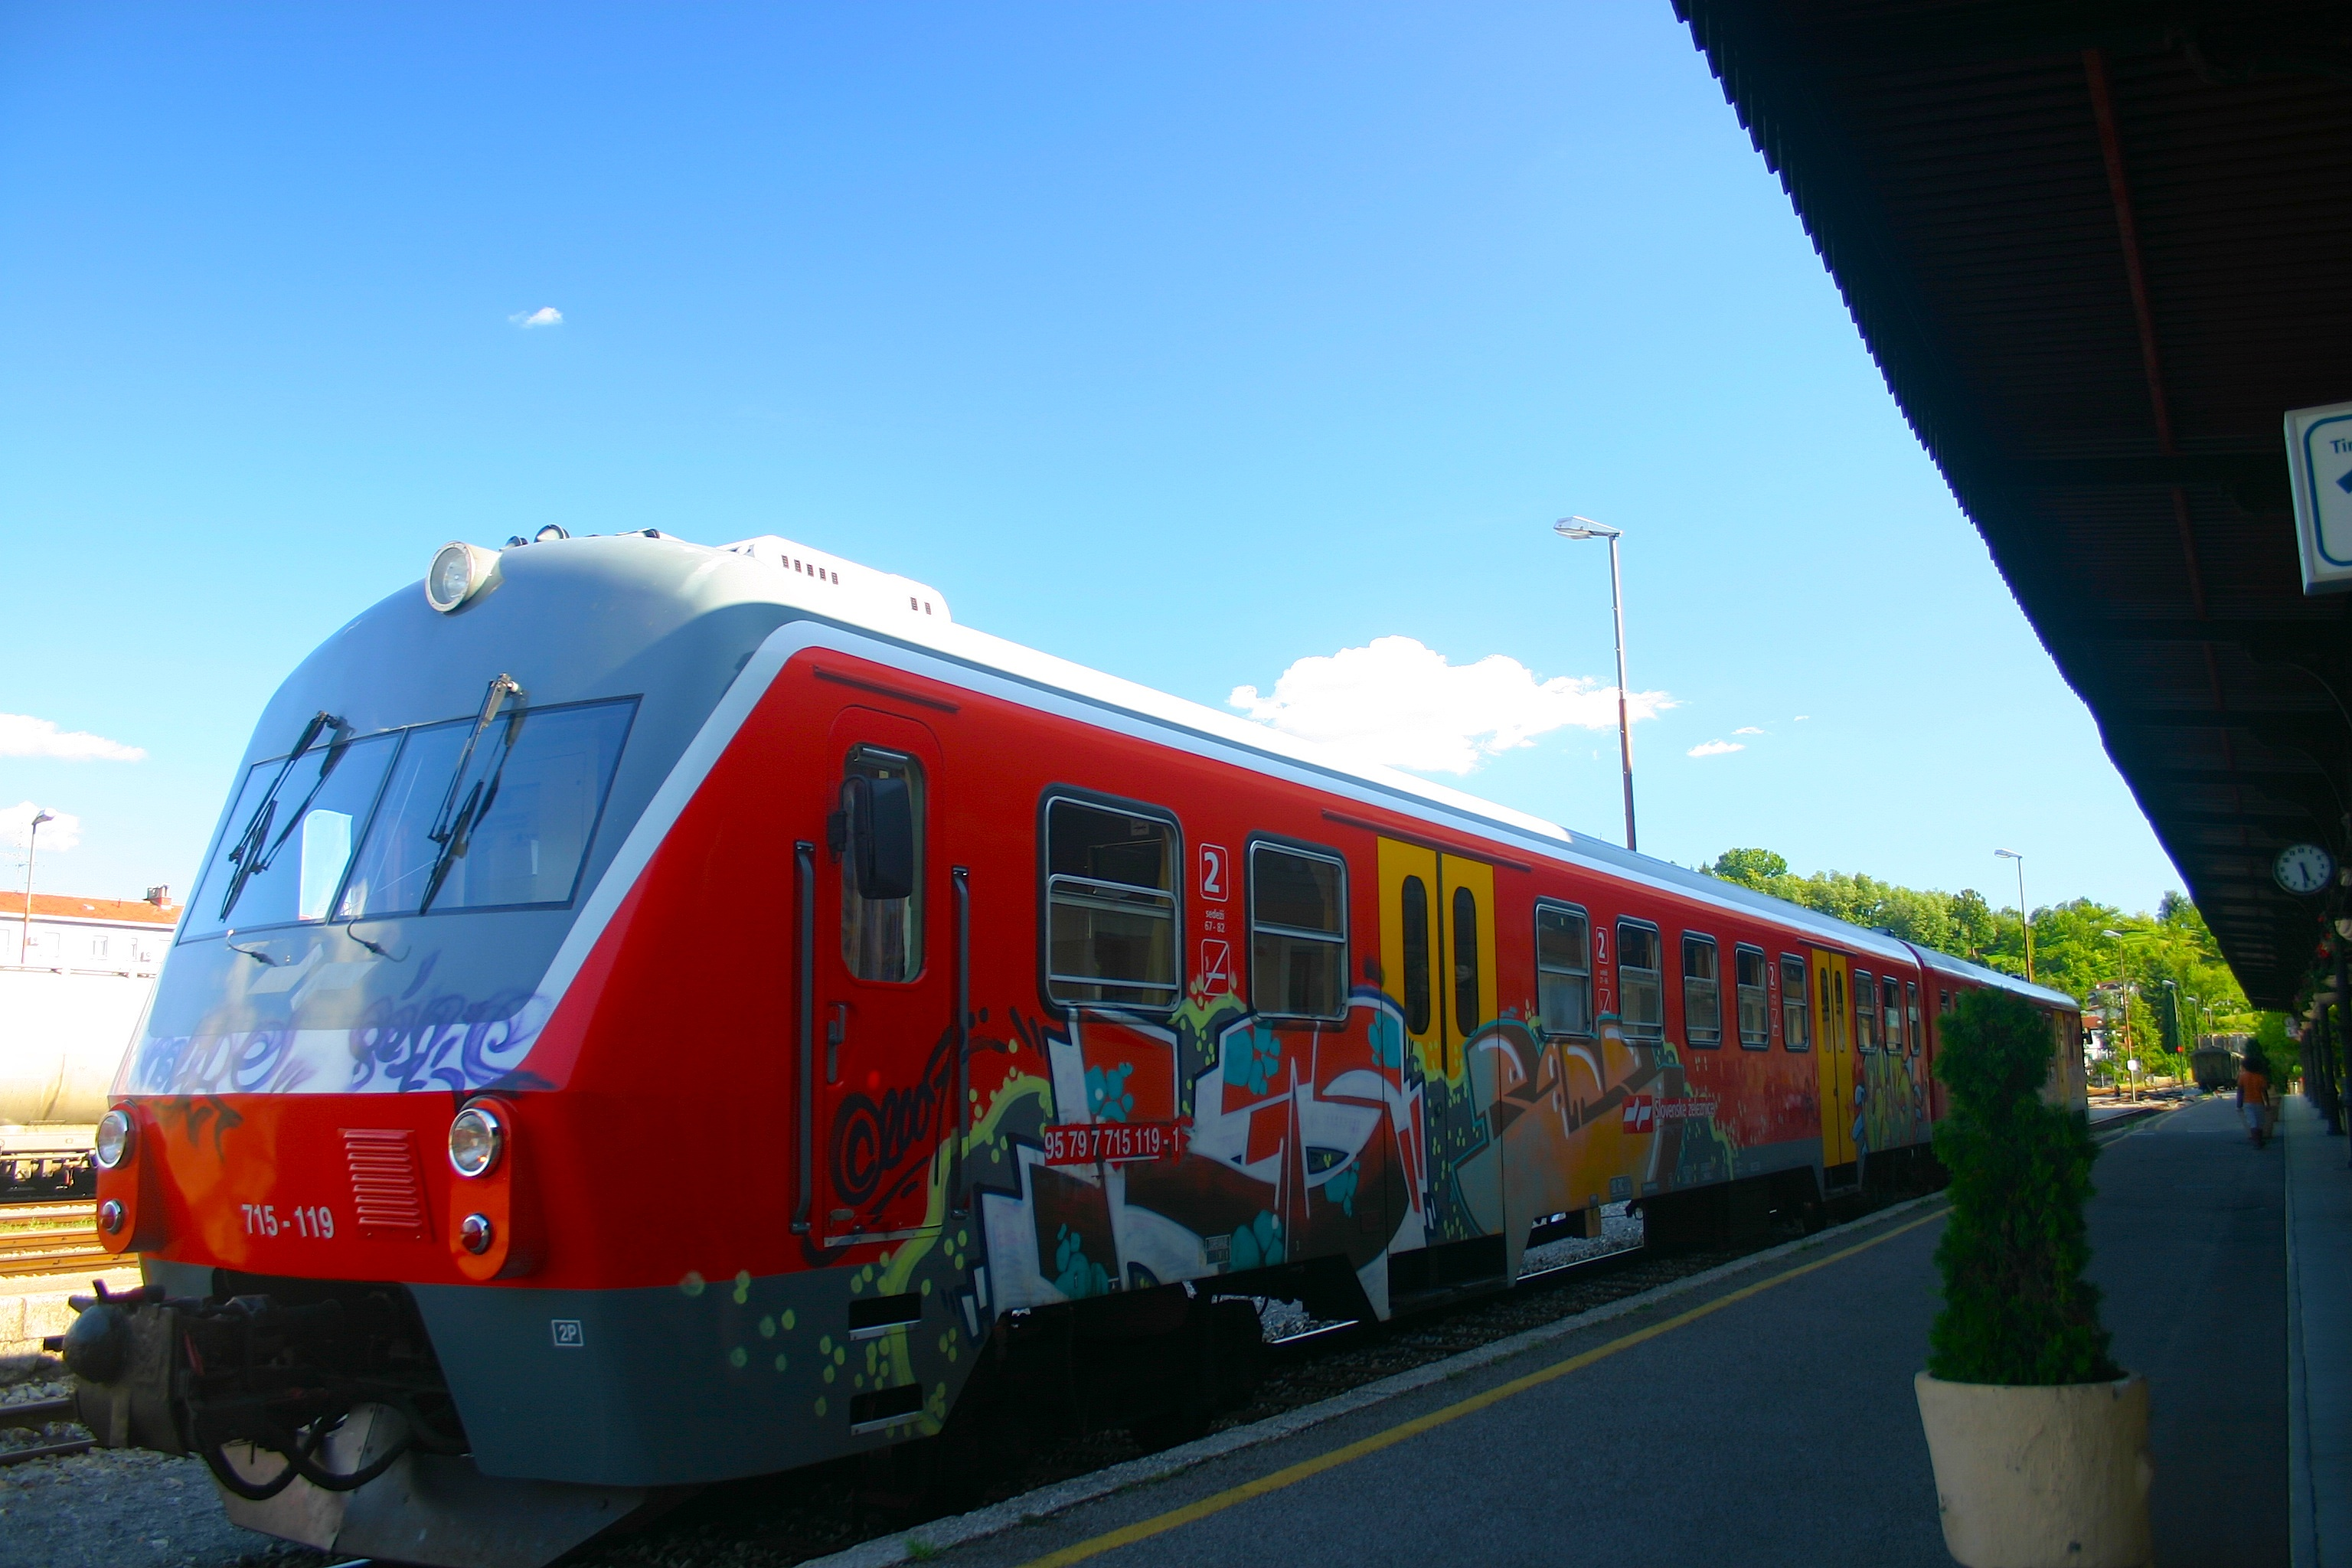
\includegraphics[width=\linewidth]{appendices/Slovenian/2009-07-26-22.36.40 - Tharatorn Supasiti - Train Journey 5 - IMG_5280-1--orig.jpg}} 
 \caption{Many expedition veterans have made their way to Tolmin via train (vlak) and/or bus (avtobus). \pic{Tharatorn Supasiti}}
 \label{Thara train}
\end{marginfigure}



\subsection{Directions}

How do I get to\ldots{}? -- Kako pridem do\ldots{}?\\
Can you show me on the map? -- Mi lahko pokažete na zemljevidu/načrtu?\\
Street -- cesta/ulica\\
Turn left. -- Zavijte levo.\\
Turn right. -- Zavijte desno.\\
left  -- levo\\
right -- desno\\
straight ahead -- naravnost\\
towards the -- proti\\
past the -- mimo\\
before the -- pred\\
Watch for the -- Bodite pozorni na\\
intersection -- križišče\\
north -- sever\\
south -- jug\\
east -- vzhod\\
west -- zahod\\
uphill -- navzgor\\
downhill –- navzdol\\

\subsection{Money}

Can you change money for me? -- Mi lahko zamenjate denar?\\
Where can I get money changed? -- Kje lahko zamenjam denar?\\
What is the exchange rate? -- Kakšno je menjalno razmerje?\\
ATM -- bankomat\\
Bank -- banka\\
exchange office -- menjalnica\\
Money -- denar\\
Cheque -- ček\\
currency -- valuta\\

\subsection{Eating}

Can I look at the menu, please? -- Lahko prinesete jedilni list?\\
I'm a vegetarian. -- Sem vegetarijanec.\\
May I have a glass of? -- Lahko dobim kozarec?\\
May I have a cup of ? -- Lahko dobim skodelico?\\
May I have a bottle of? -- Lahko dobim steklenico?\\
Excuse me, waiter? -- Natakar!\\
I'm finished. -- Končal sem.\\
It was delicious. -- Bilo je odlično.\\
The check, please. -- Račun, prosim.\\
inn -- gostilna\\
snack bar -- okrepčevalnica\\
pizzeria -- picerija\\
breakfast -- zajtrk\\
lunch -- malica/kosilo\\
supper -- večerja\\
meal -- obrok\\
soup -- juha\\
appetizer -- aperitiv\\
hors d'oeuvre -- predjed\\
main course -- glavna jed\\
desert -- sladica\\
snack -- prigrizek\\

\subsection{Food}


\begin{marginfigure}
\checkoddpage \ifoddpage \forcerectofloat \else \forceversofloat \fi
\centering
 \frame{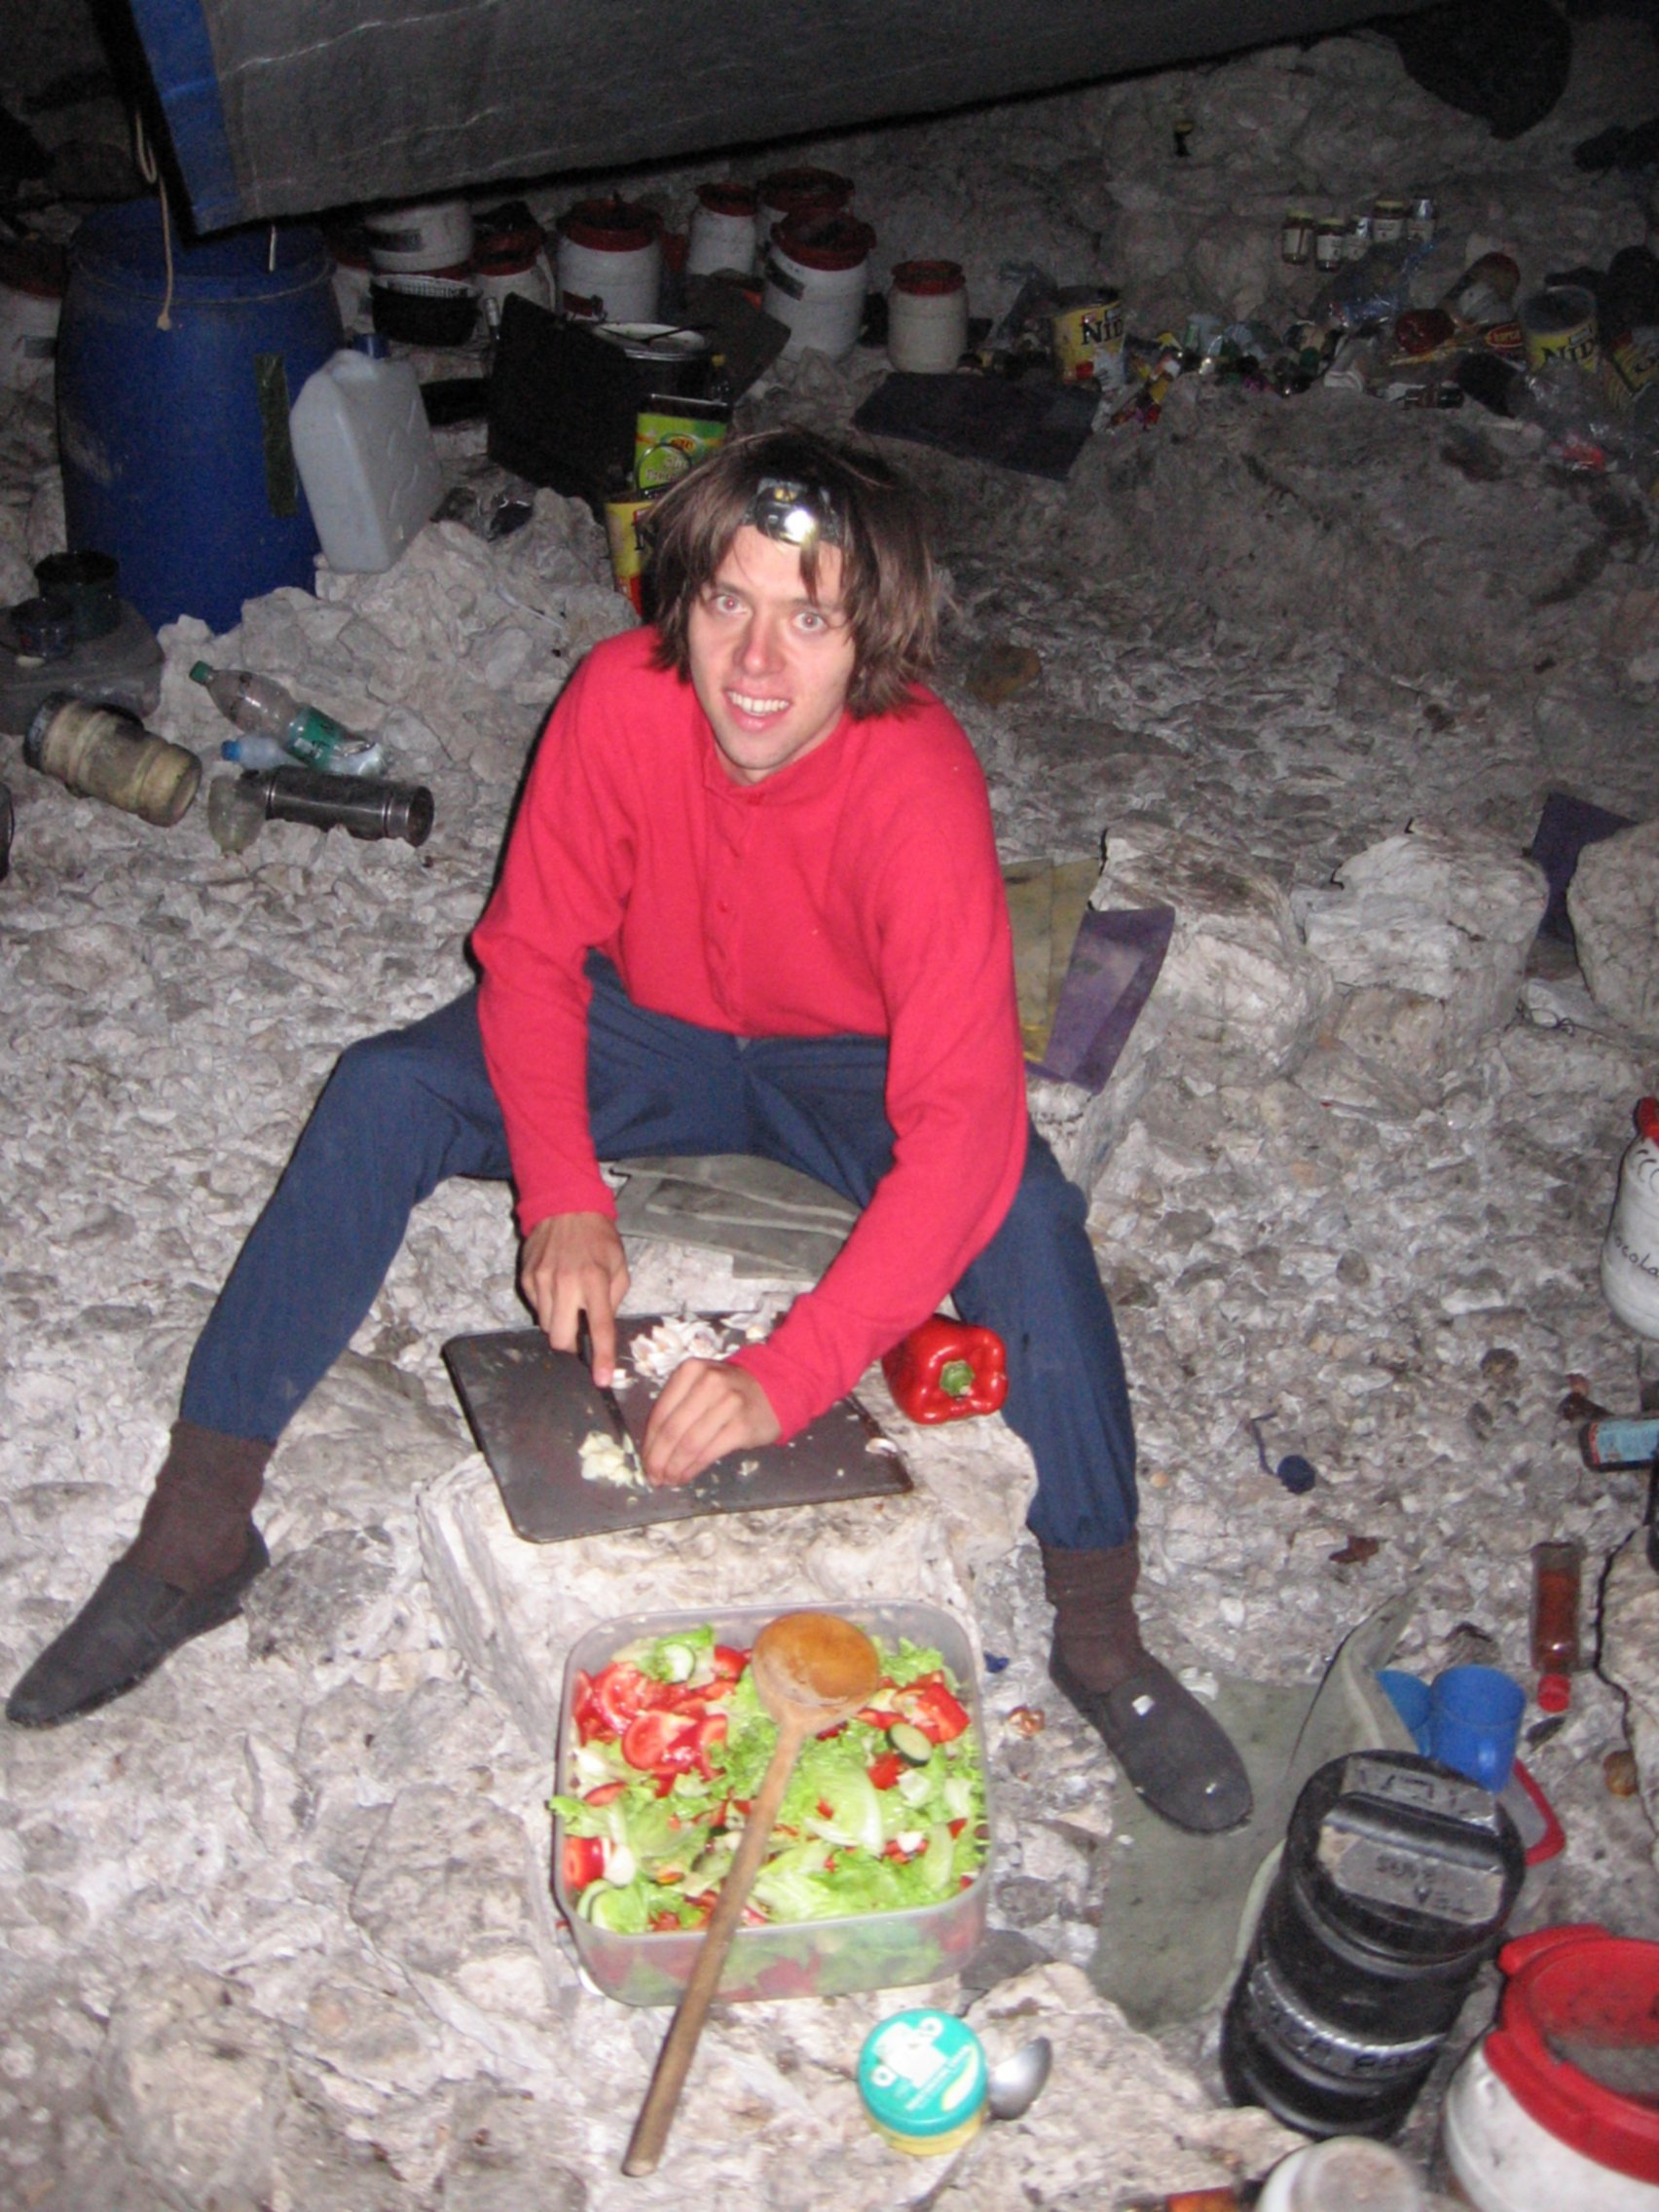
\includegraphics[width=\linewidth]{appendices/Slovenian/jarvist frost - bruno the bivi salad master--orig.jpg}} 
 \caption{Bruno was "the bivi salad (solata) master" of 2007. \pic{Jarvist Frost}}
 \label{solata}
\end{marginfigure}

chicken -- piščanec\\
beef -- govedina\\
fish -- riba\\
ham -- šunka\\
sausage -- klobasa\\
cheese -- sir\\
eggs -- jajca\\
salad -- solata\\
vegetables -- zelenjava\\
fruit -- sadje\\
bread -- kruh\\
croissant -- rogljiček\\
donut -- krof\\
noodles -- rezanci/testenine\\
rice -- riž\\
beans -- fižol\\
salt -- sol\\
black pepper -- črni poper\\
butter -- maslo\\
Deep fried cheese –- Pohan sir\\

\subsection{In a bar}

\begin{marginfigure}
\checkoddpage \ifoddpage \forcerectofloat \else \forceversofloat \fi
\centering
 \frame{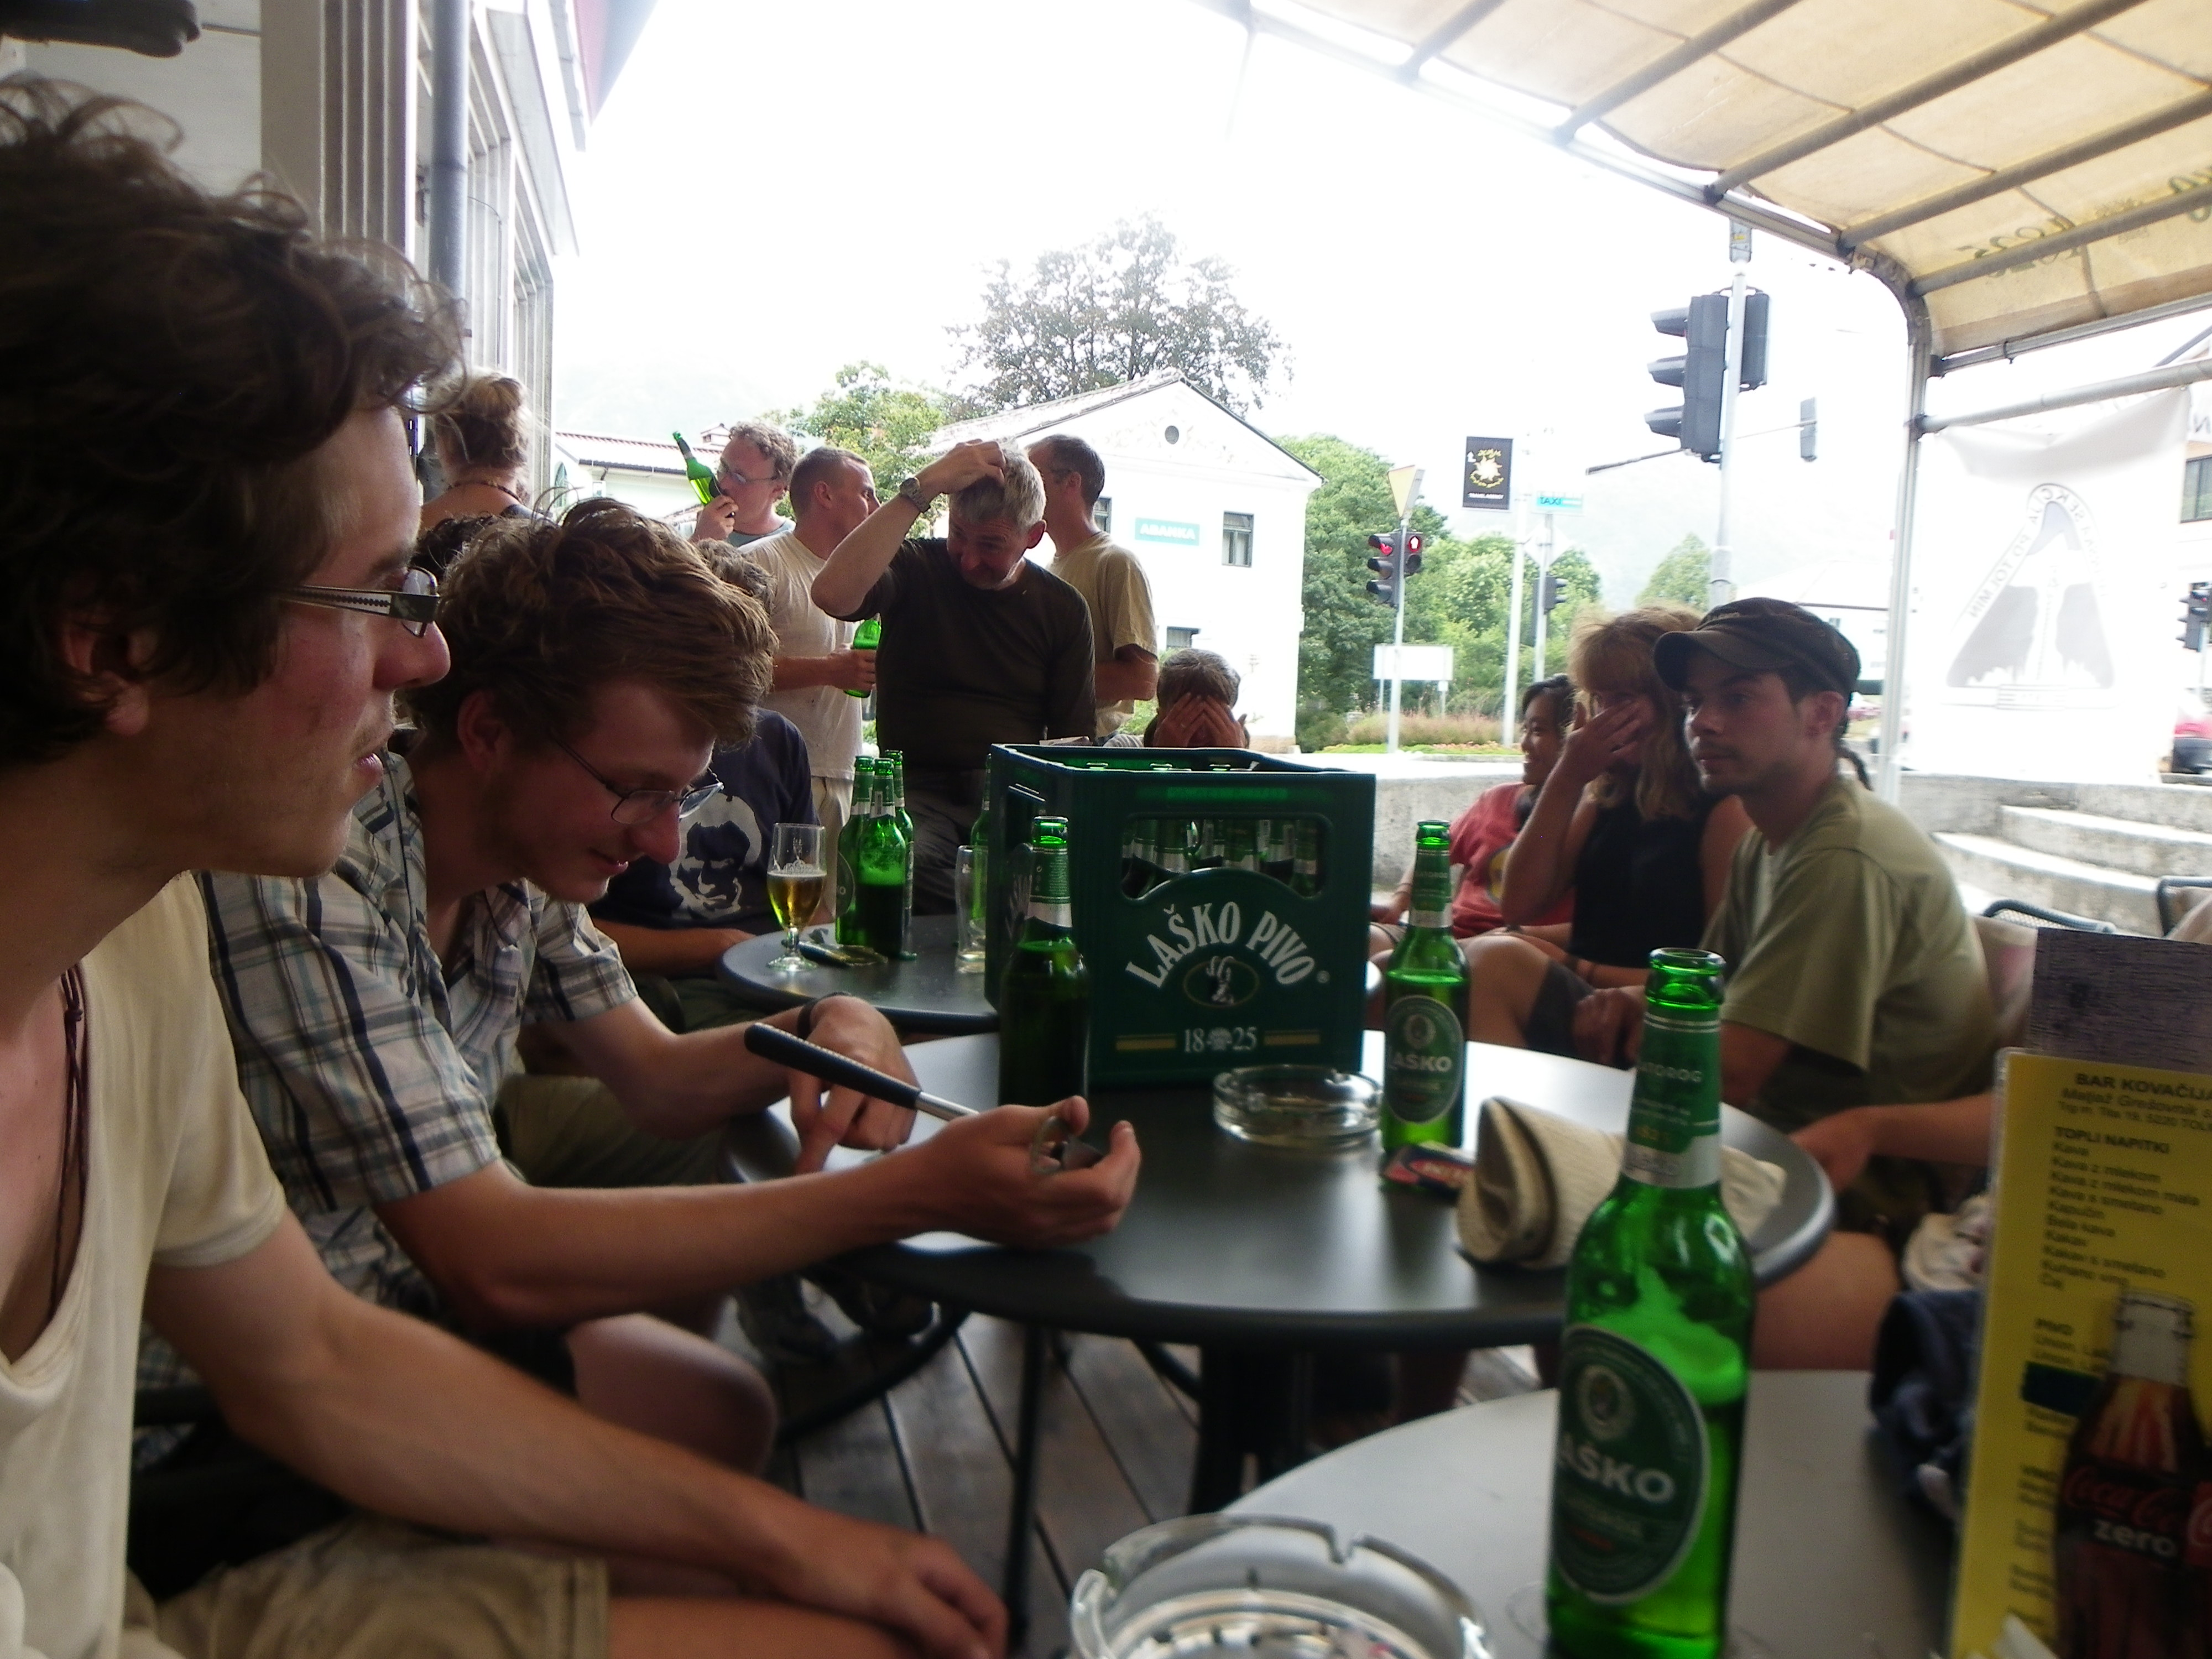
\includegraphics[width=\linewidth]{appendices/Slovenian/2012-08-16-19.04.11-Rhys Tyers-Pentax X90-IMGP3432--orig.jpg}} 
 \caption{Beer! (Pivo!) \pic{Rhys Tyers}}
 \label{pivo}
\end{marginfigure}

Do you serve alcohol? -- Ali strežete žgane pijače?\\
A beer/two beers, please. -- Pivo/dve pivi, prosim.\\
A glass of red/white wine, please. -- Kozarec rdečega/belega vina, prosim.\\
A pint, please. -- Veliko pivo, prosim.\\
A bottle, please. -- Steklenico, prosim.\\
Do you have any bar snacks? -- Imate kakšne prigrizke?\\
One more, please. -- Še enega/eno, prosim.\\
Another round, please. -- Še enkrat enako, prosim.\\
When is closing time? -- Kdaj zaprete?\\
whiskey -- viski\\
vodka -- vodka\\
rum -- rum\\
water -- voda\\
orange juice - pomarančni sok\\
Coke - kokakola\\
Tea – čaj\\
Coffee – kava\\

\begin{marginfigure}
\checkoddpage \ifoddpage \forcerectofloat \else \forceversofloat \fi
\centering
 \frame{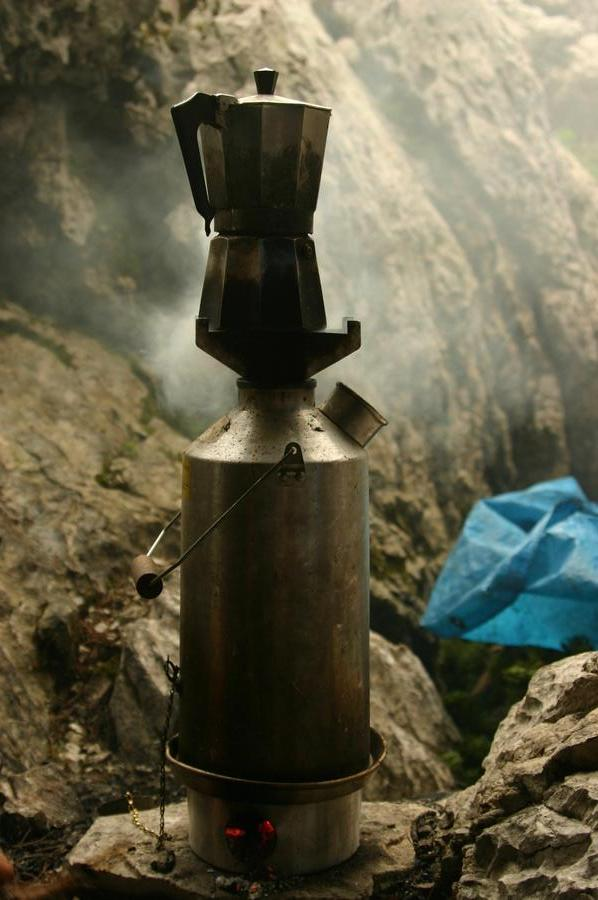
\includegraphics[width=\linewidth]{appendices/Slovenian/Gergely Ambrus - DSLR - img_4879--orig.jpg}} 
 \caption{Making coffee (kava) on the Kelly Kettle (don't try this at home). \pic{Gergely Ambrus}}
 \label{kava}
\end{marginfigure}


\subsection{Shopping}

How much is this?  -- Koliko stane to?\\
expensive  -- drago\\
cheap  -- poceni\\
I don't want it.  -- Tega nočem.\\
You're cheating me.  -- Hočete me ogoljufati.\\
I'm not interested.  -- Ne zanima me.\\
OK, I'll take it.  -- Dobro, vzel bom to.\\
Can I have a bag?  -- Lahko dobim vrečko?\\
I need\ldots{}  -- Potrebujem\ldots{}\\


\subsection{Driving}

no parking -- parkiranje prepovedano\\
speed limit -- omejitev hitrosti\\
gas (petrol) station -- bencinska črpalka\\
petrol -- bencin\\
diesel -- dizelsko gorivo\\
traffic sign -- prometni znak\\
traffic lights -- semafor\\
road -- cesta\\
fee -- kazen\\
detour -- obvoz\\
Bicycle -– kolo\\
street -- cesta/ulica\\
square/circus -- trg\\
pavement -- pločnik\\
driver -- voznik\\
pedestrian -- pešec\\


\begin{marginfigure}
\checkoddpage \ifoddpage \forcerectofloat \else \forceversofloat \fi
\centering
 \frame{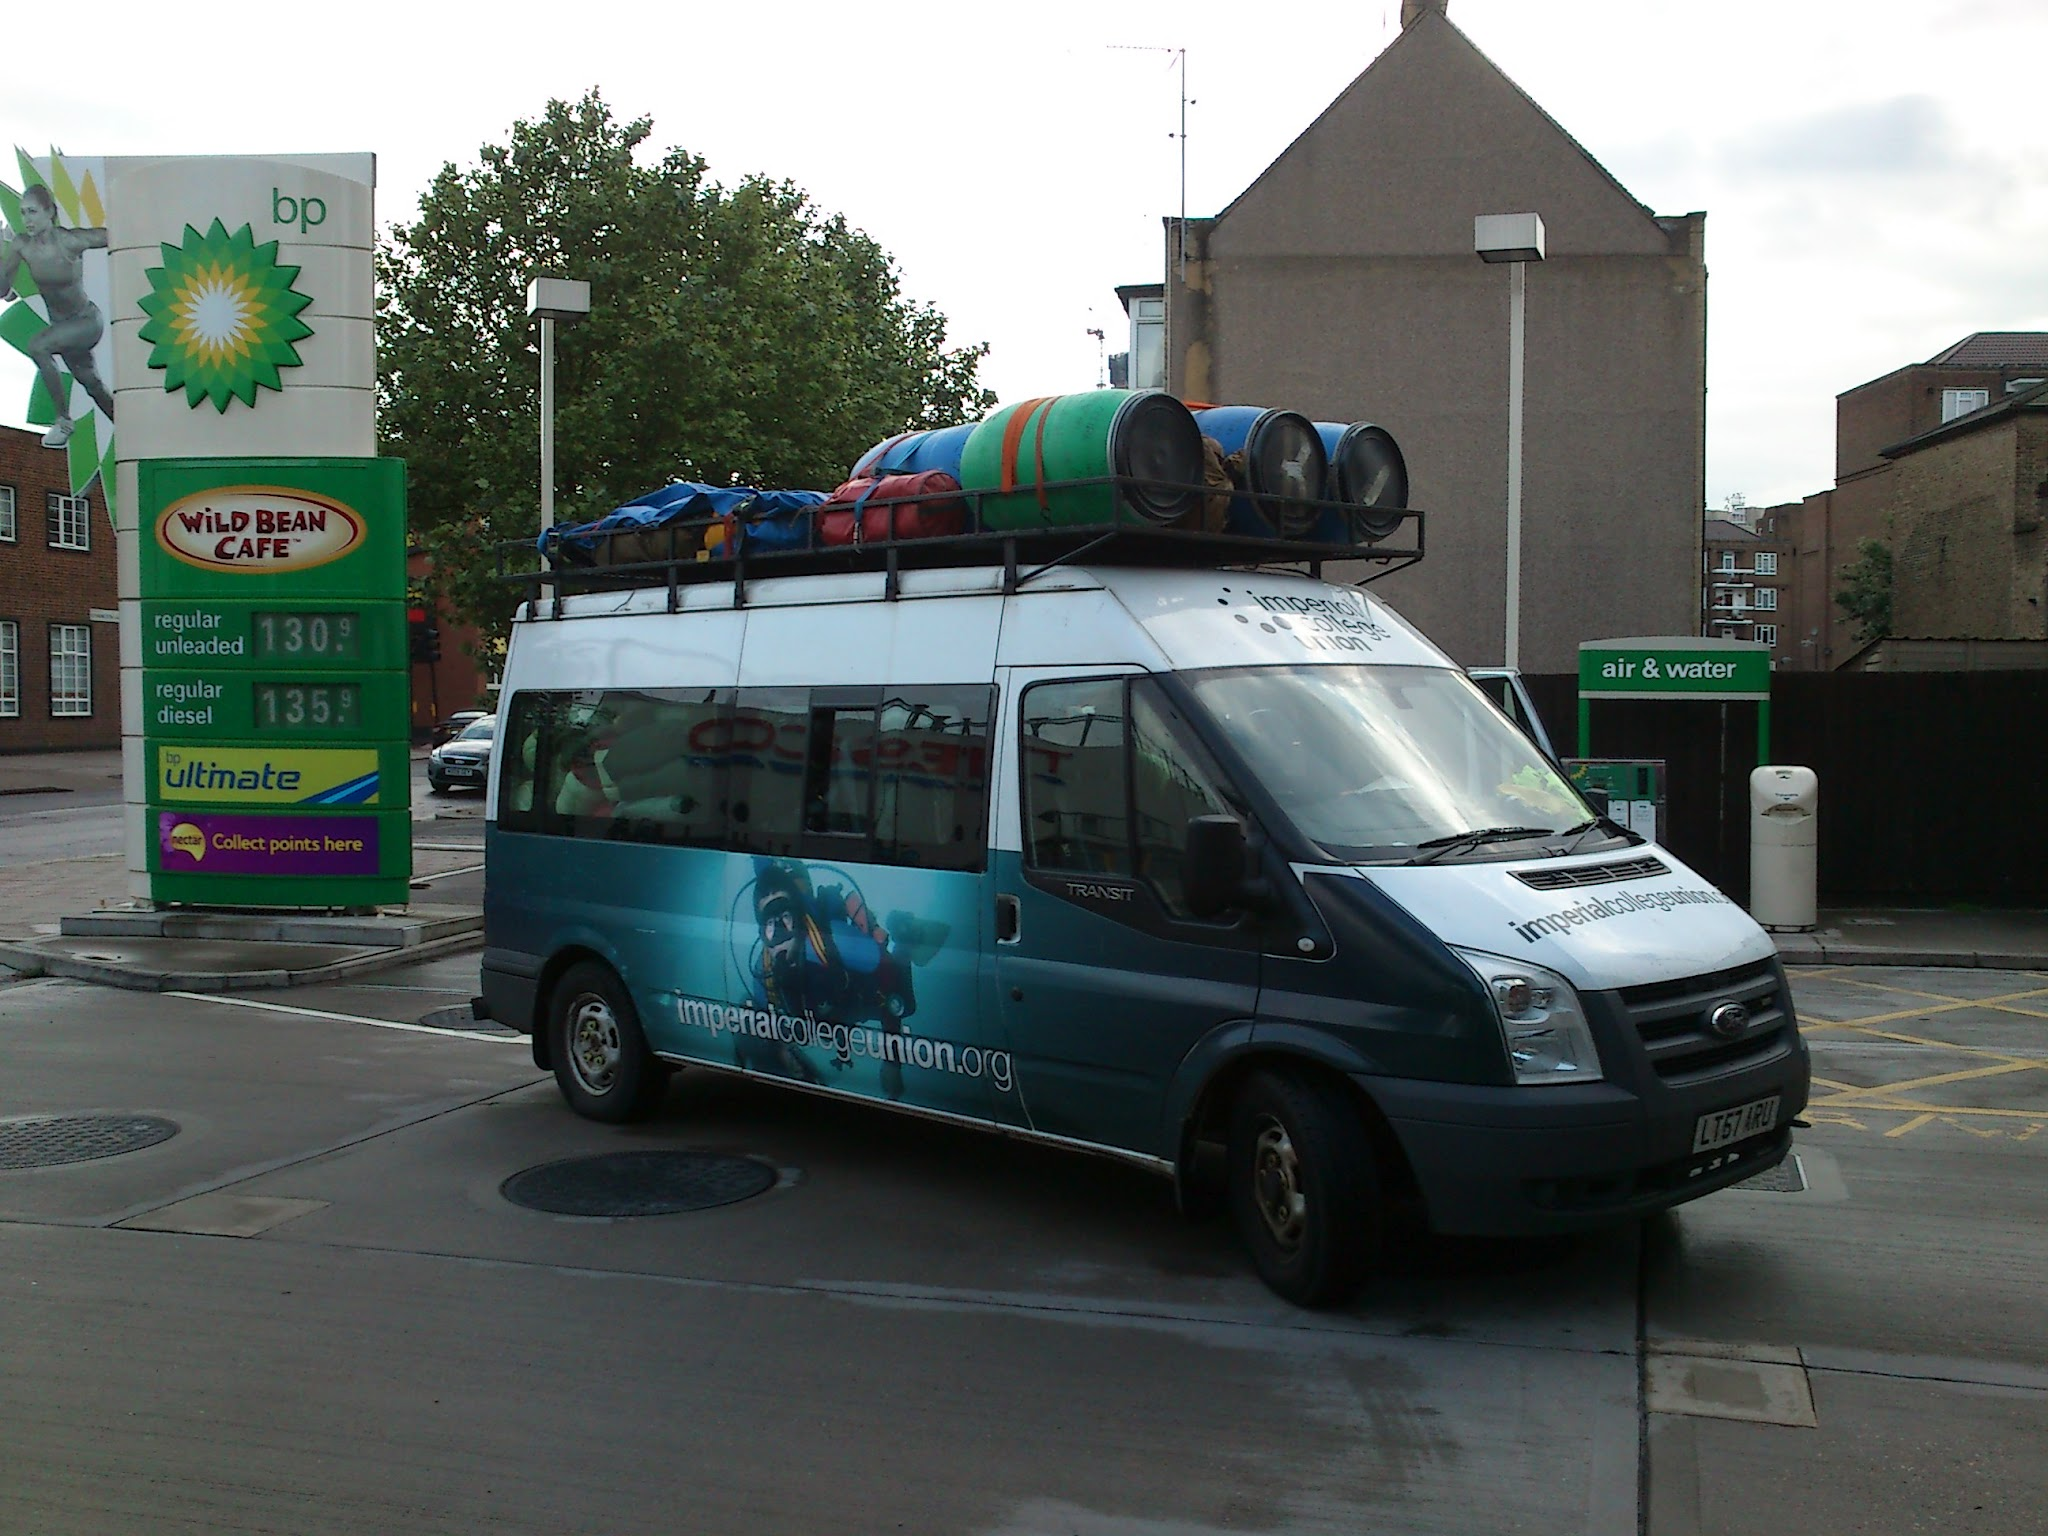
\includegraphics[width=\linewidth]{appendices/Slovenian/2012-07-13-1850JarvistMooreFrost-DSC_0262--orig.jpg}} 
 \caption{The minibus, loaded and ready to go, fuelling up in an English petrol station (bencinska črpalka). \pic{Jarvist Frost}}
 \label{petrol station}
\end{marginfigure}

\subsection{Grammar}

\textbf{Singular}\\
Jaz -- I\\
Ti -- you\\
On –- he / Ona –- she\\
\textbf{Plural}\\   
Midva –- us two\\
Vidva –- the two of us\\
Onadva –- both of them\\
\textbf{Dual}\\
Mi –- we\\
Vi –- all of you\\
Oni –- those\\
\textbf{Masculine}\\
On -- he\\
brat -- brother\\
oče -- father\\
\textbf{Feminine}\\
ona -- she\\
sestra -- sister\\
mati -- mother\\
\textbf{Neutral}\\
ono -- it\\
dete -- child\\
telo –- body\\


\begin{marginfigure}
\checkoddpage \ifoddpage \forcerectofloat \else \forceversofloat \fi
\centering
 \frame{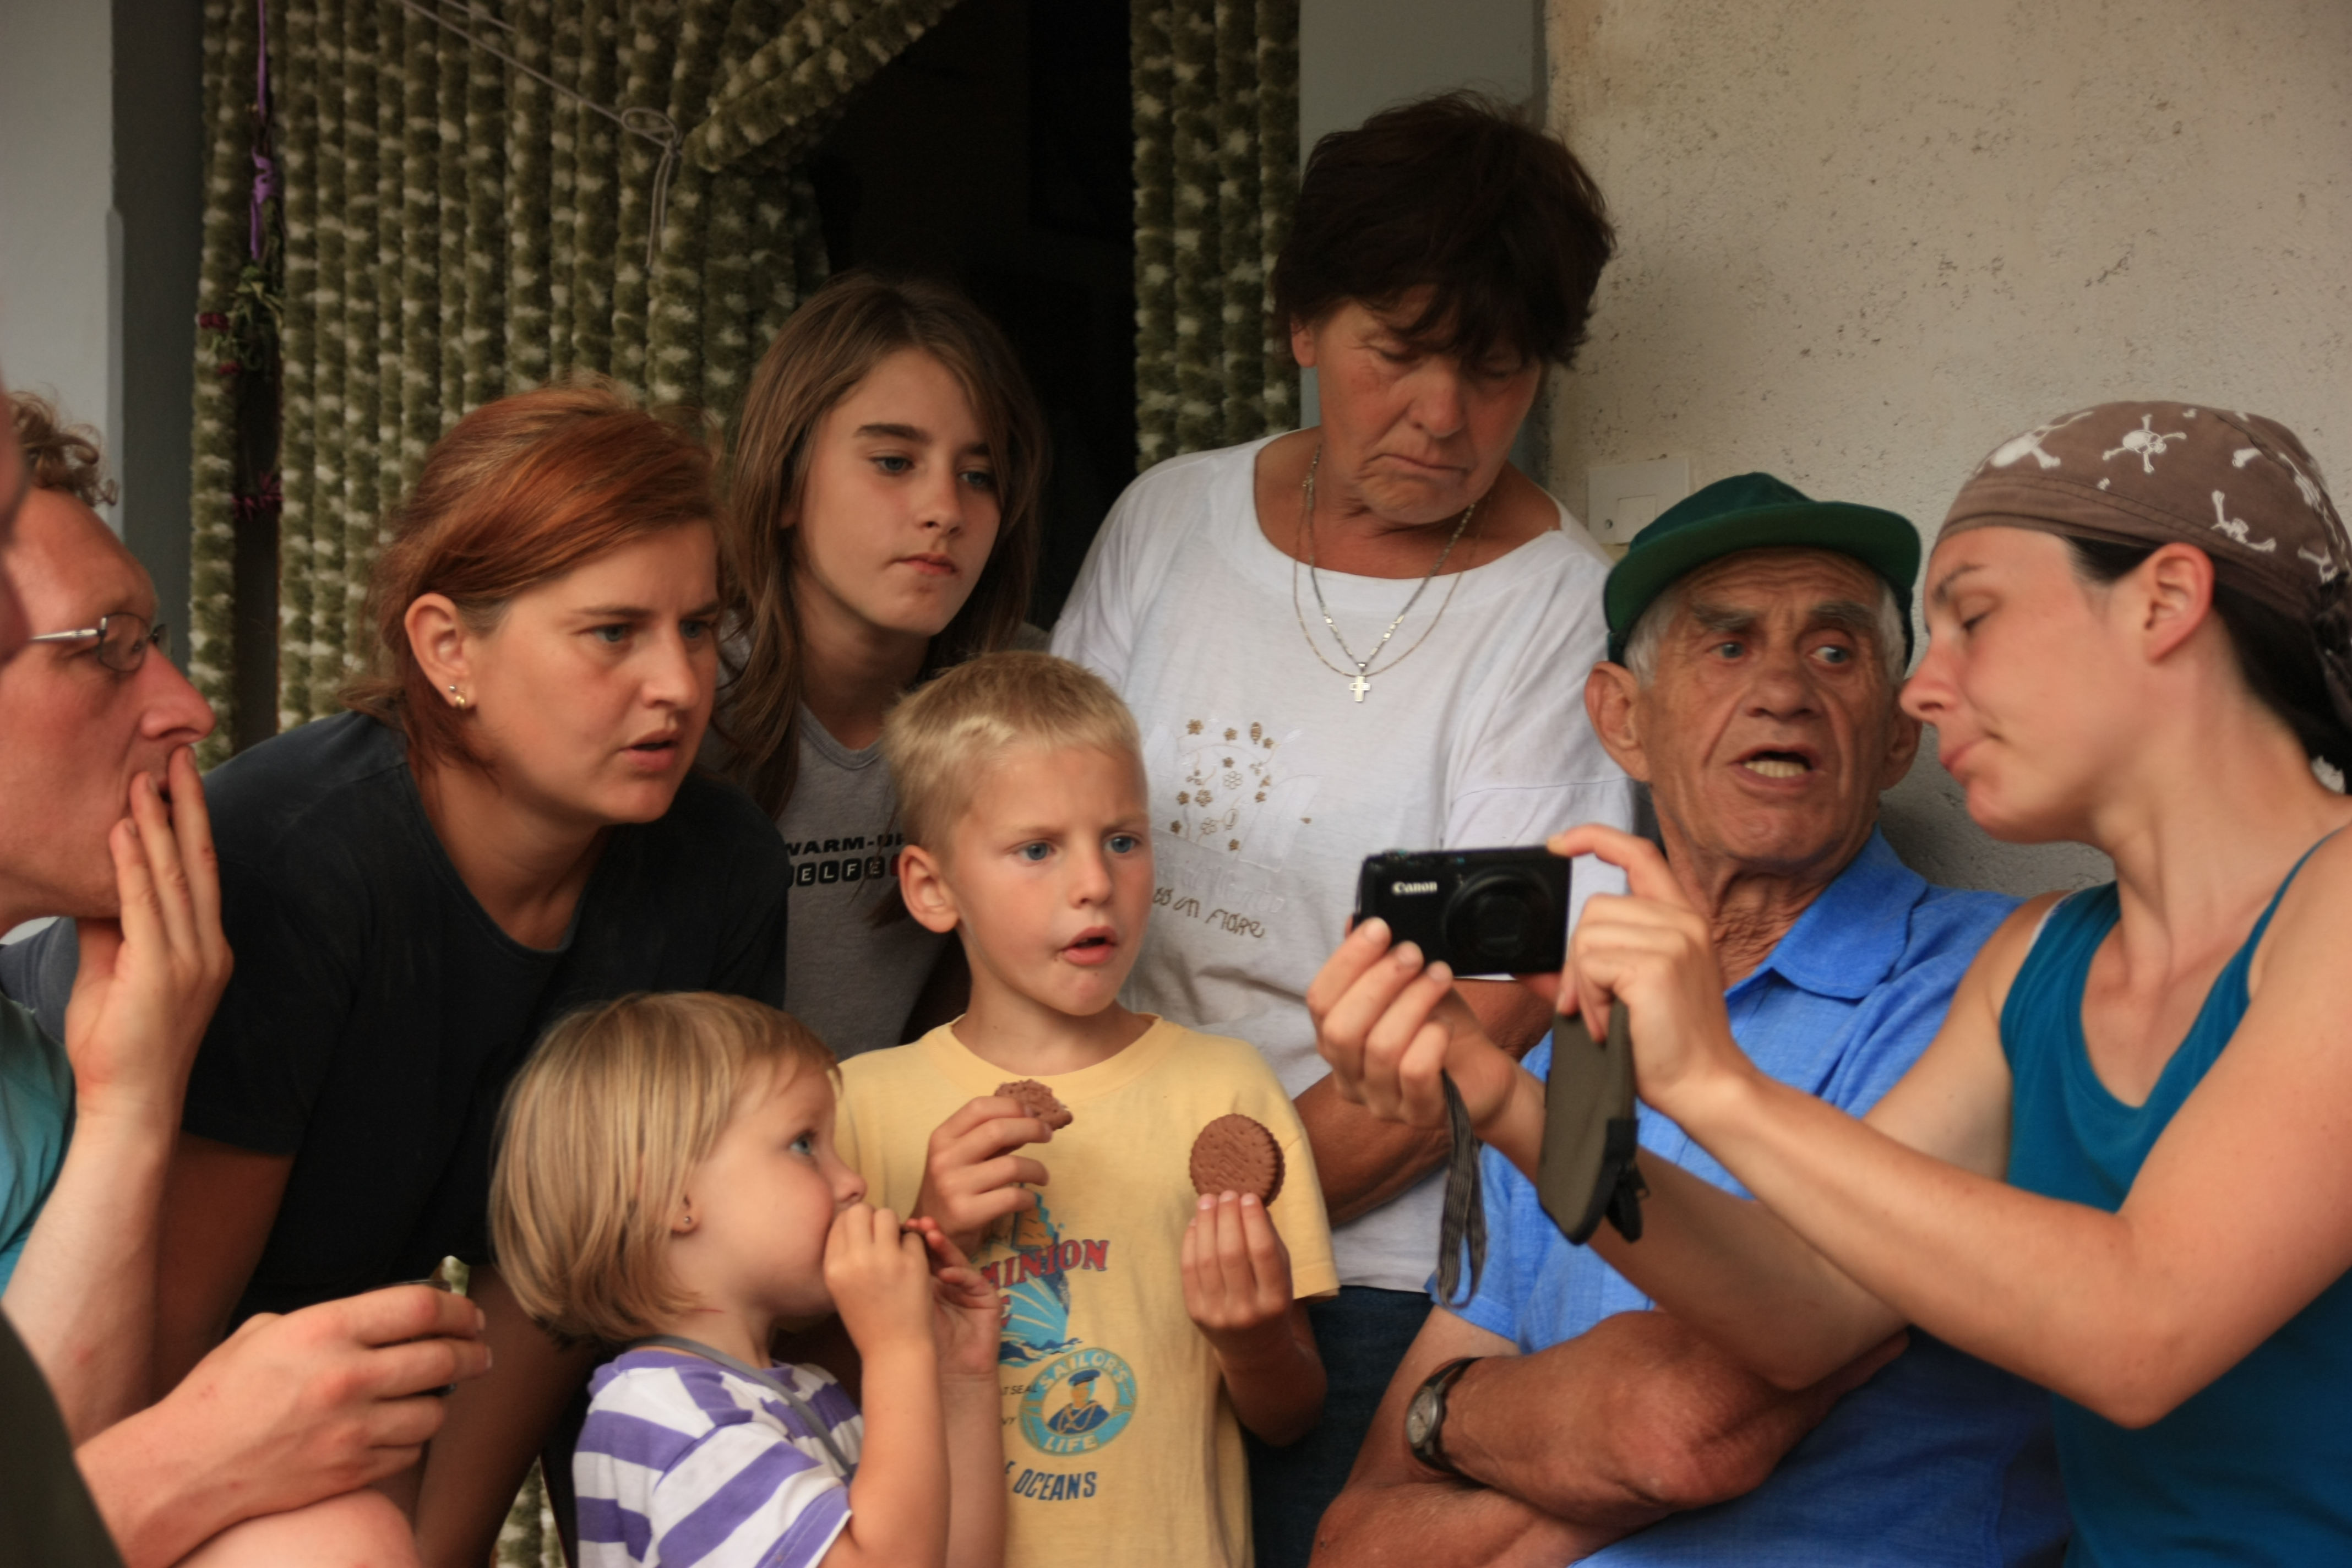
\includegraphics[width=\linewidth]{appendices/Slovenian/2012-08-16-0654-GergelyAmbrus-IMG_2627--orig.jpg}} 
 \caption{Jana showing photographs to the Skalar family (and Jim, far left) in Ravne after the successful connection. \pic{Gergely Ambrus}}
 \label{skalar camera}
\end{marginfigure}

